\chapter{Analisi di Steiner (secondo Giannì)}
\nocite{Steiner1953}

L'introduzione dell'analisi di Downs stimolò diversi ricercatori e clinici a sviluppare le proprie analisi: quello che ne seguì fu una proliferazione di marker cefalometrici che non fecero altro che confondere i clinici. Cecil C. Steiner selezionò quelli che per lui erano i parametri più significativi, e sviluppò un'analisi che credeva potesse fornire il massimo numero di informazioni cliniche con il minor numero di misurazioni.

Vennero quindi scelte alcune misure, e furono determinate delle medie statistiche su un numero di pazienti normo-occlusi.

Nell'analisi delle teleradiografie latero-laterali, Steiner propose la valutazione separata di varie parti del cranio, nello specifico i tessuti scheletrici, i tessuti dentali e i tessuti molli. L'analisi scheletrica si propone di porre in relazione la mascella e la mandibola tra di loro e con le ossa del cranio. L'analisi dentale mette in relazione gli incisivi superiori e inferiori con le rispettive basi ossee e tra di loro. Infine, l'analisi dei tessuti molli fornisce un mezzo per valutare il bilanciamento e l'armonia del profilo facciale inferiore\footcite{Steiner1953,Steiner1959,Steiner1960}.

A cavallo tra gli anni '70 e '80, Ennio Giannì\footcite{Gianni1980} propose diverse aggiunte all'analisi di Steiner. A tutt'oggi, questa è la tecnica più utilizzata, data la relativa semplicità e velocità d'esecuzione.

\begin{table}[h]
%\footnotesize
\caption{Punti specifici introdotti da Giannì}
\begin{tabularx}{\textwidth}{>{\textit}clX}
\toprule
%\multicolumn{3}{l}{\textbf{Punti di repere}} \\
%\midrule
D & Centro della sinfisi mentoniera & Punto di incontro del massimo diametro orizzontale con il massimo diametro verticale. \\
SOr & Sopraorbitario & Punto di incontro del tetto dell'orbita con il margine esterno dell'orbita stessa.\\
IST & Pavimento della sella & Il punto più basso del contorno della sella turcica. \\
\bottomrule
\end{tabularx}
\end{table}

\section{Analisi scheletrica}
\begin{table}[h]
%\footnotesize
\begin{tabularx}{\textwidth}{>{\bfseries}lXc}
\toprule
 & Punti di riferimento & Valore medio\\
\cmidrule(r){2-3}
Angolo \angolo{SNA} &  & 82° $\pm$ 2° \\
Angolo \angolo{SNB} &  & 80° $\pm$ 2° \\
Angolo \angolo{ANB} &  & 2° $\pm$ 2° \\
Angolo cranio-spinale & piano \piano{S}{N} -- piano bispinale & 10° $\pm$ 3° \\
Angolo cranio-occlusale & piano occlusale -- \piano{S}{N} & 14° $\pm$ 3° \\
Angolo cranio-mandibolare & piano mandibolare -- \piano{S}{N} & 32° $\pm$ 5° \\
Angolo intermascellare & piano bispinale -- piano mandib. & 20° $\pm$ 5° \\
Angolo occluso-spinale & piano occlusale -- piano bispinale & 8° $\pm$ 2° \\
Angolo occluso-mandibolare & piano occlusale -- piano occlusale & 12° $\pm$ 3° \\
Base cranica posteriore & piano \piano{S}{N} -- piano \piano{S}{Ba} & 129° $\pm$ 5° \\
Angolo cranio-sinfisario & piano \piano{S}{N} -- piano \piano{N}{D} & 76° $\pm$ 3° \\
\bottomrule
\end{tabularx}
\end{table}

Nelle analisi antropologiche tradizionali, così come nell'analisi di Downs, il piano di riferimento era il \textit{piano di Francoforte}. Sulle teleradiografie latero-laterali è però spesso difficile identificare i punti Porion e Orbitale, per la determinazione di tale piano. Steiner scelse quindi la \textbf{base cranica anteriore} (Sella-Nasion) come piano di riferimento della sua analisi. Il vantaggio di utilizzare due punti ``mediani'' è che si muovono minimamente quando la testa devia dalla posizione di profilo, o quando la testa ruota nel cefalostato.

\begin{figure}[p!]
\subfloat[][]
   {\label{fig:steiner_sna}\fbox{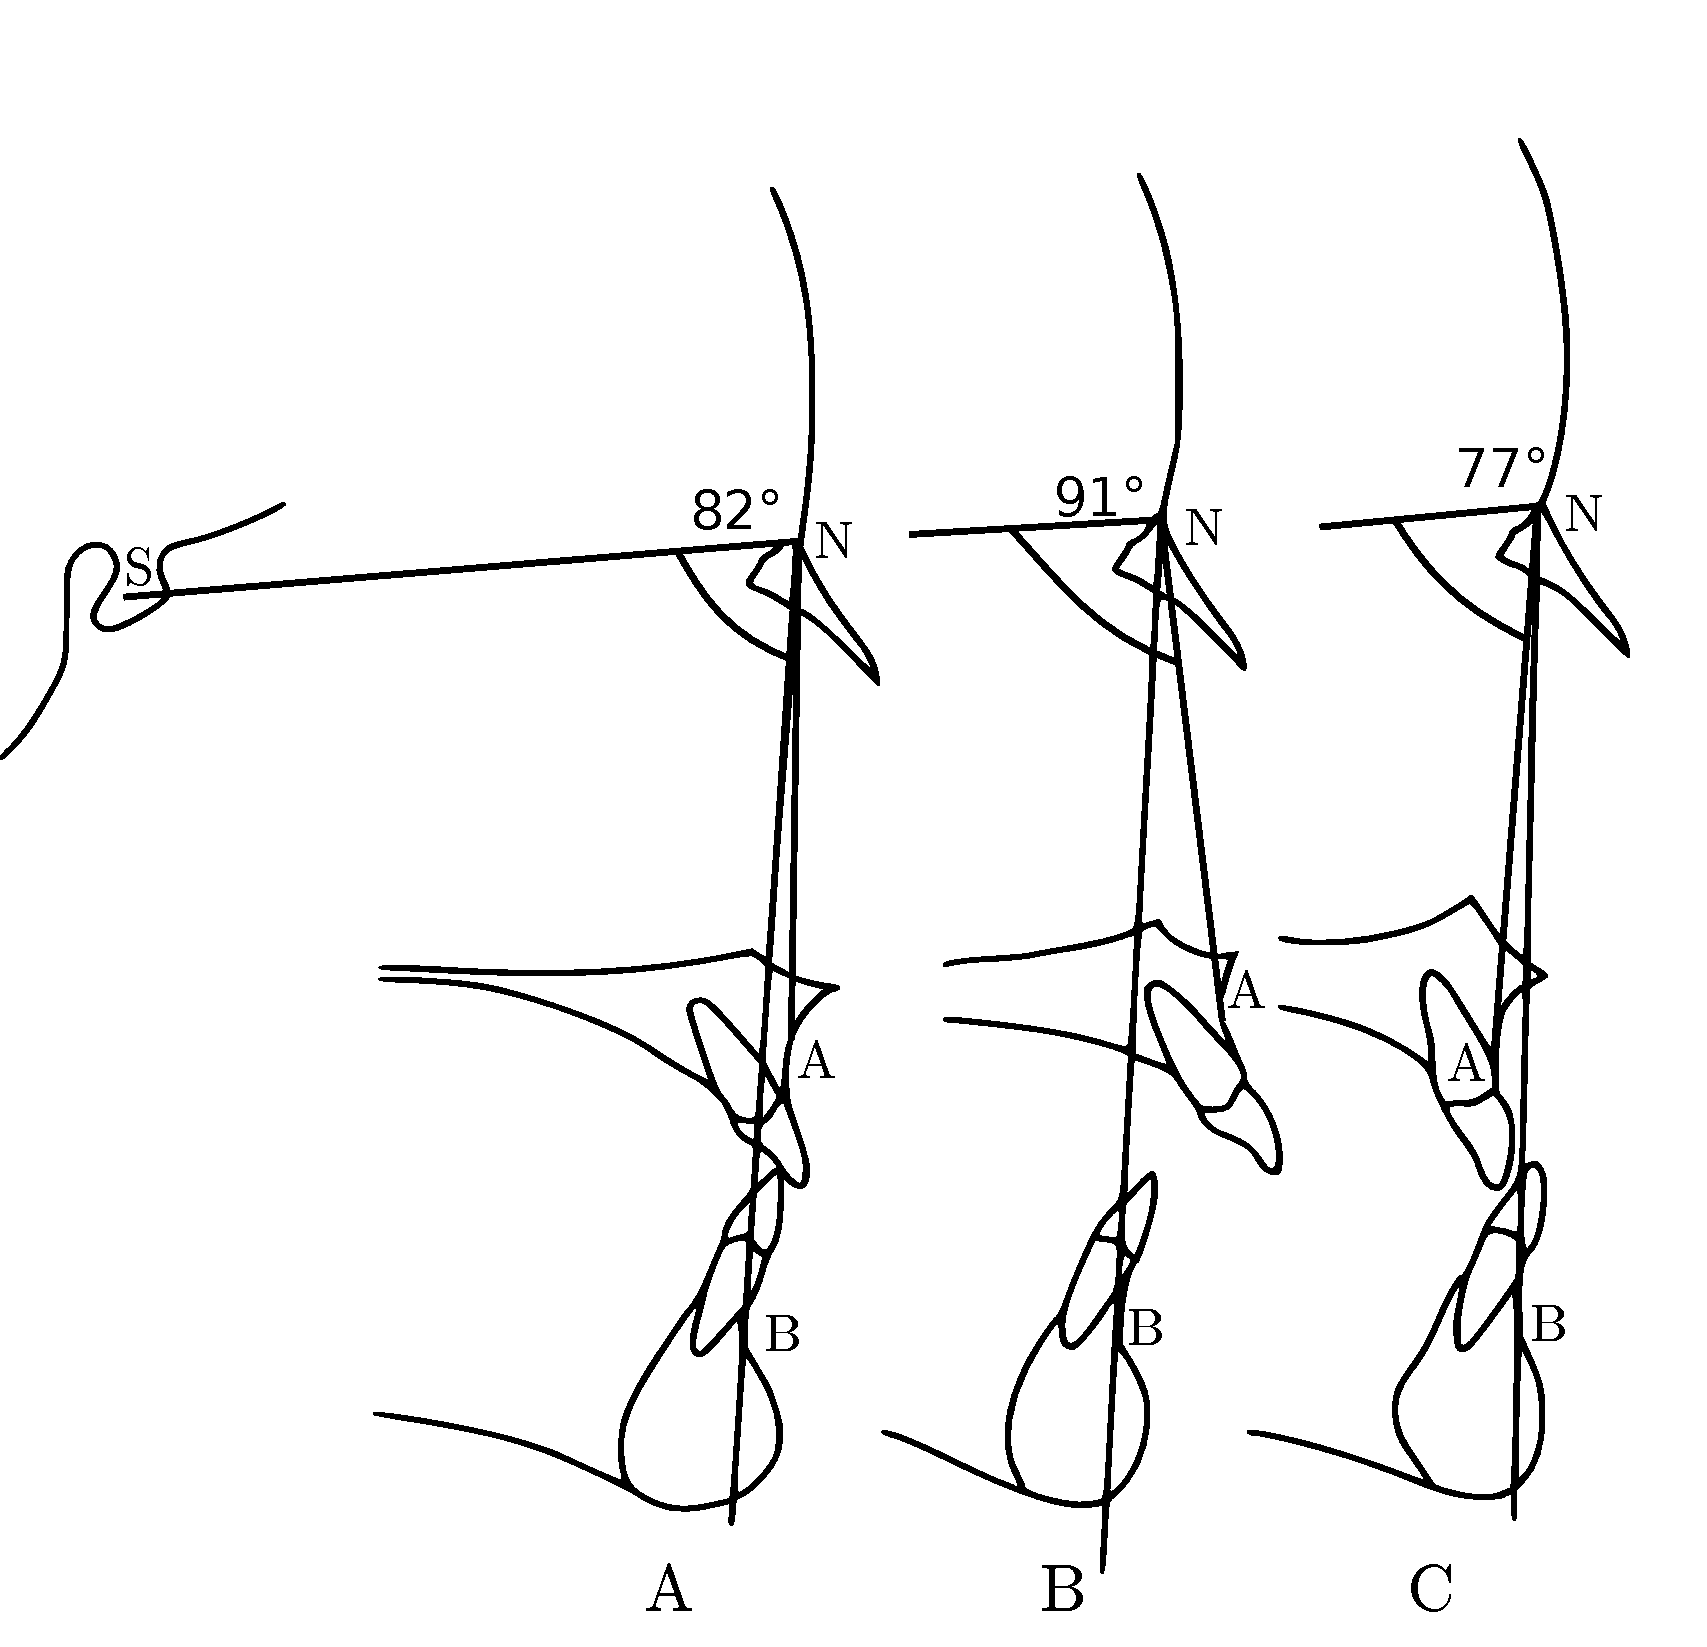
\includegraphics[width=.45\textwidth]{./images/steiner_sna.pdf}}} \quad
\subfloat[][]
   {\label{fig:steiner_snb}\fbox{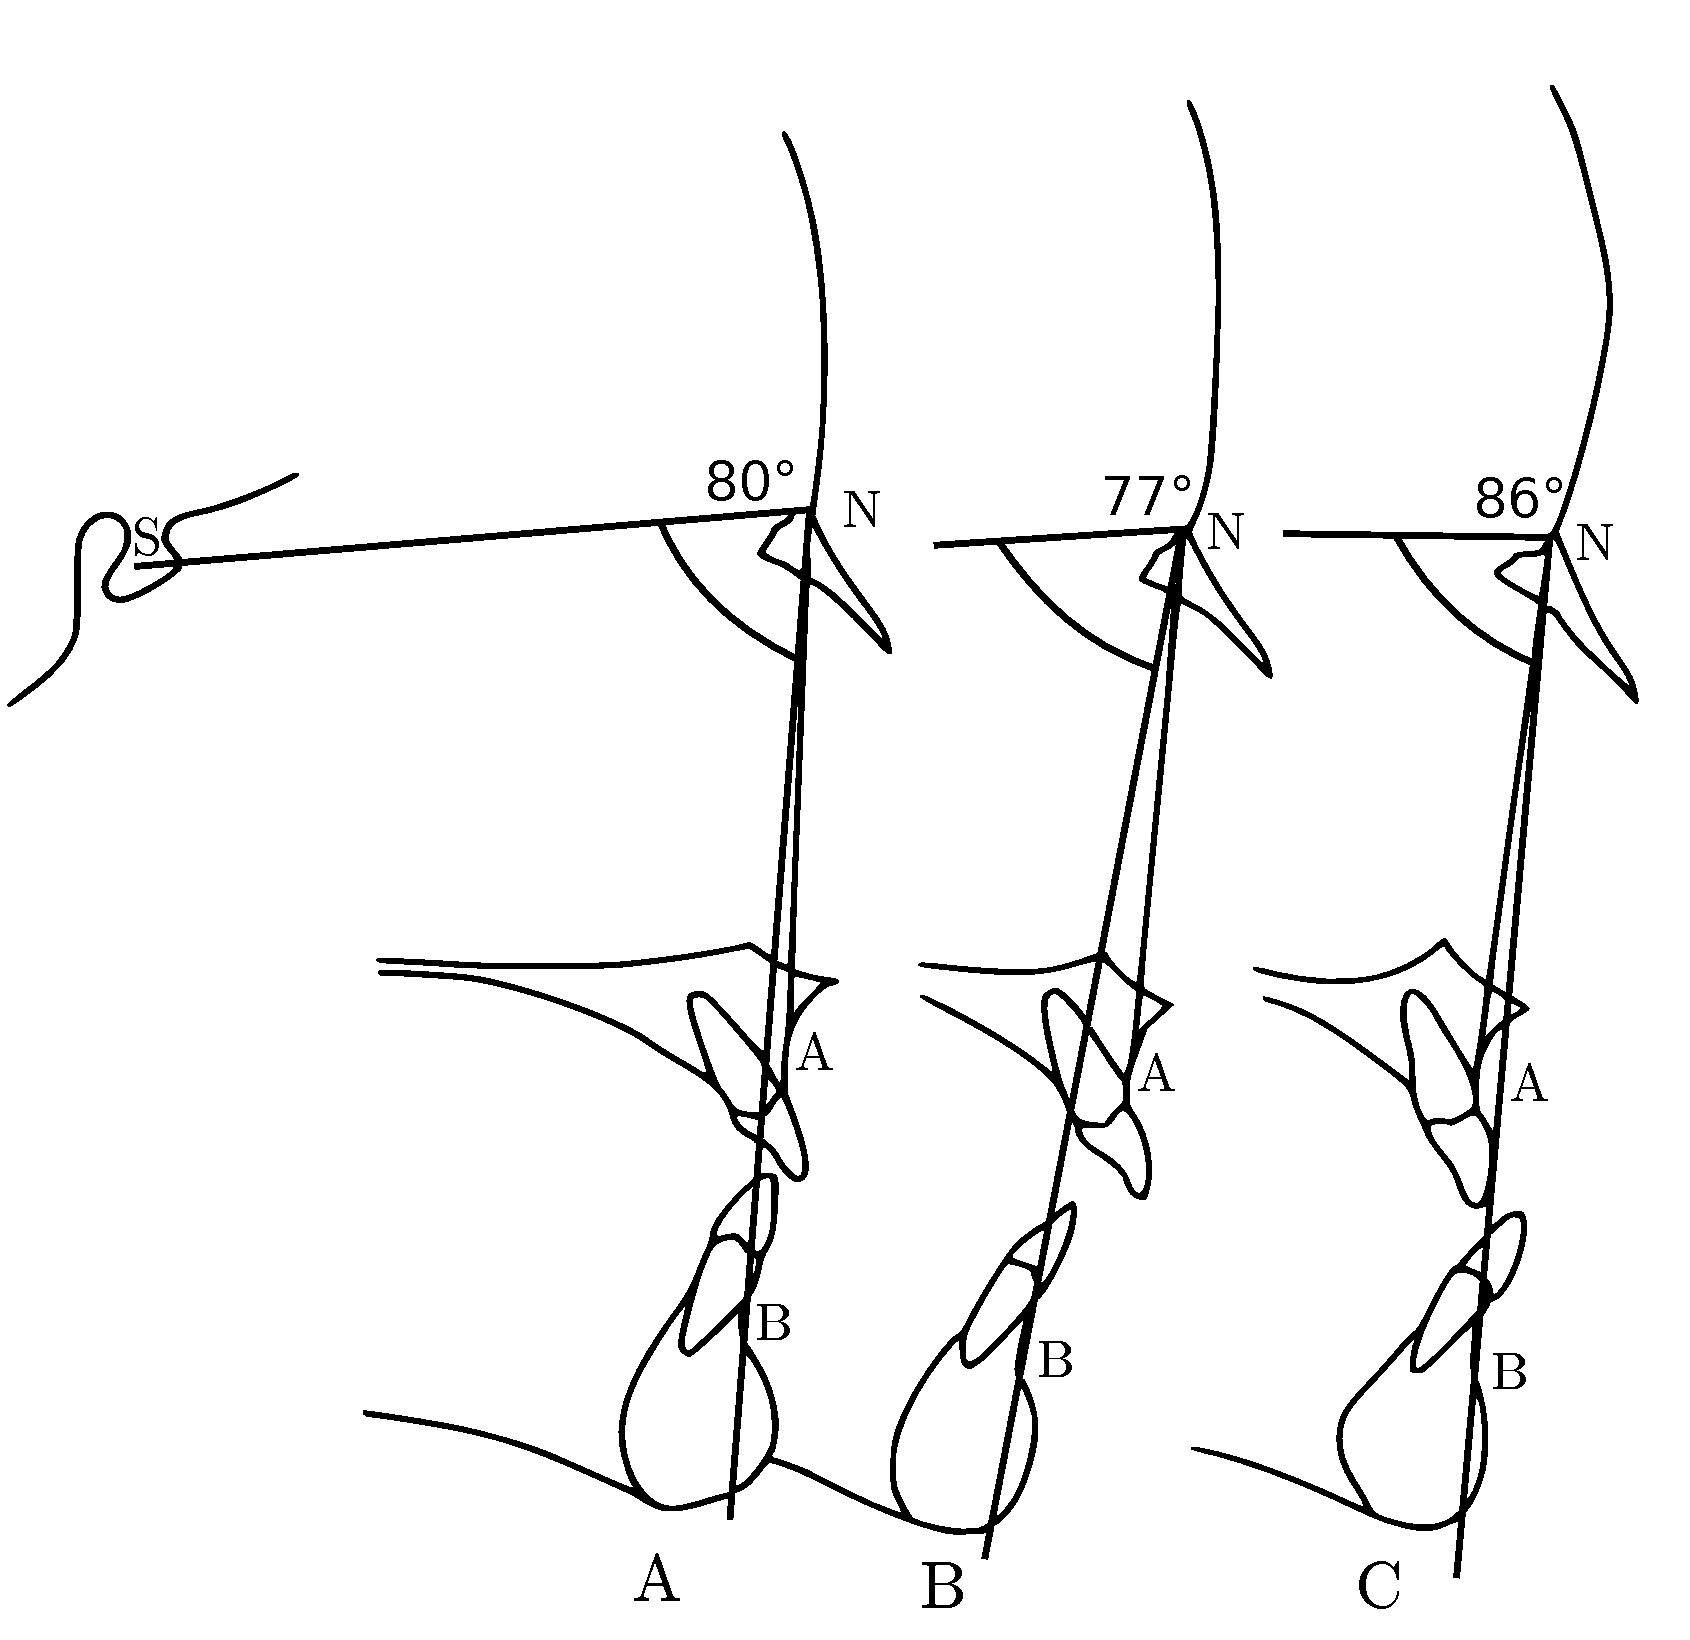
\includegraphics[width=.45\textwidth]{./images/steiner_snb.pdf}}}
 \centering
 % steiner_sna.jpg: 1024x988 pixel, 72dpi, 36.12x34.85 cm, bb=0 0 1024 988
 \caption{\subref{fig:steiner_sna} \angolo{SNA}: mascella normale, mascella protrusa, mascella retrusa. \subref{fig:steiner_snb} \angolo{SNB}: mandibola normale, mandibola retrusa, mandibola protrusa.}
 \label{fig:steiner_sna_snb}
\end{figure}
\begin{figure}[p!]
 \centering
 \fbox{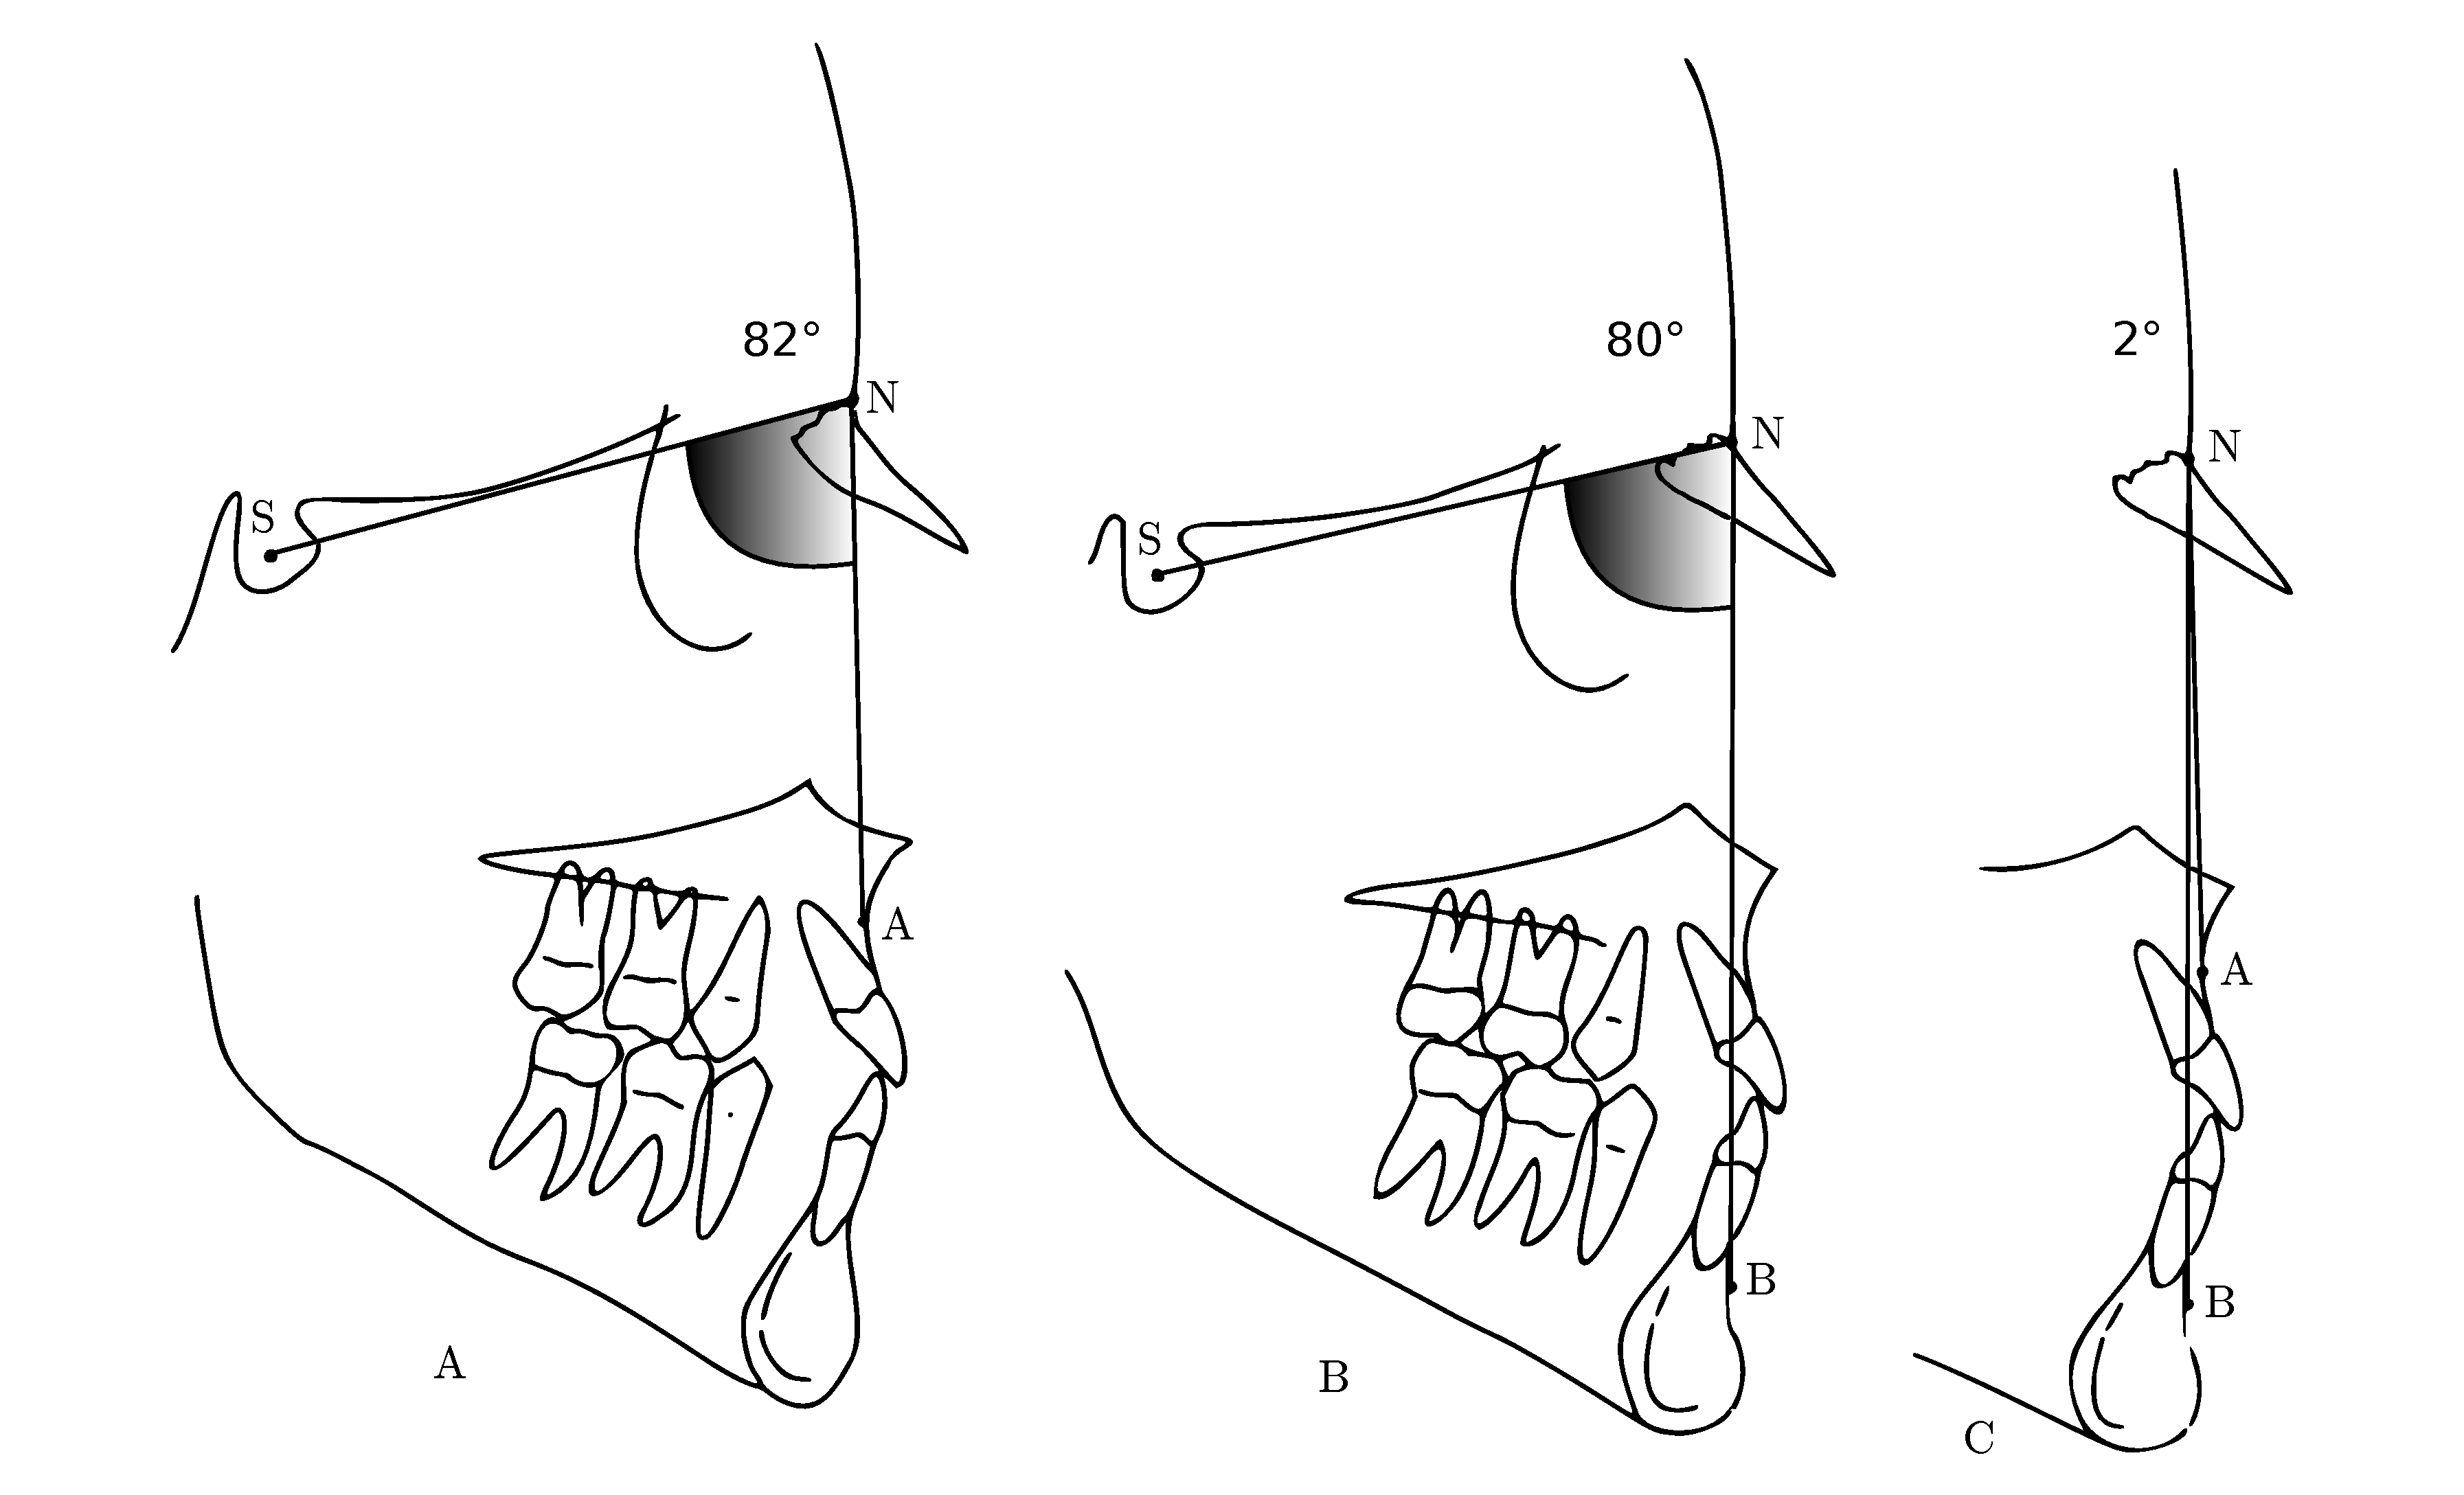
\includegraphics[width=.9\textwidth]{./images/steiner_anb.pdf}}
 % steiner_anb.jpg: 2152x1306 pixel, 72dpi, 75.92x46.07 cm, bb=0 0 2152 1306
 \caption{l'angolo interincisale \angolo{ANB} è dato dalla differenza tra \angolo{SNA} e \angolo{SNB}.}
 \label{fig:steiner_anb}
\end{figure}

\paragraph{Mascella (angolo \angolo{SNA})}
I punti A e B vengono considerati come i limiti anteriori delle basi apicali di, rispettivamente, mascella e mandibola. Perciò, per determinare la posizione della mascella rispetto alla base cranica, viene calcolato l'angolo \angolo{SNA}, il cui valore medio è 82° $\pm$ 2° (fig.~\vref{fig:steiner_sna}). Se il valore angolare è maggiore, la mascella si trova in posizione anteriore rispetto alla base cranica. Di contro, se il valore inferiore, la mascella si troverà posizionata posteriormente.

\paragraph{Mandibola (angolo \angolo{SNB})}
Per valutare la posizione della mandibola, viene calcolato l'angolo \angolo{SNB} (valore medio 80° $\pm$ 2°, fig.~\ref{fig:steiner_snb}). Un angolo minore indica una mandibola retrusa, un angolo maggiore indica una mandibola protrusa.

\paragraph{Relazione tra mascella e mandibola (\angolo{ANB})}
Valutando i valori \angolo{SNA} e \angolo{SNB}, solitamente è possibile riconoscere il segmento osseo malposizionato. Il valore più significativo è, comunque, l'angolo \angolo{ANB}, che fornisce informazioni sulla posizione dei due segmenti ossei uno relativo all'altro (fig.~\vref{fig:steiner_anb}).

Steiner sosteneva come \angolo{SNA} non fosse importante quanto \angolo{SNB} e \angolo{ANB}, in quanto indica solamente una retrusione o protrusione rispetto alla base del cranio. Piuttosto, è più importante la discrepanza tra mascella e mandibola. Il valore medio dell'angolo \angolo{ANB} è di 2° $\pm$ 2°: un valore maggiore indica una \textit{tendenza} alla \textit{Classe II scheletrica}, e più è grande questo valore, più difficile sarà correggere la malocclusione. Valori minori dell'angolo, e valori sotto lo zero, indicano che la mandibola è protrusa rispetto alla mascella, suggerendo una \textit{Classe III scheletrica}.

\paragraph{Angolo cranio-spinale} considerato da Giannì, rappresenta l'inclinazione del mascellare superiore nei confronti della base del cranio. È l'angolo compreso tra il piano \piano{S}{Na} e il piano bispinale \piano{SNA}{SNP}. Ha un valore medio di 10° $\pm$ 3°. Valori minori depongono per un'antero-rotazione del piano bispinale: il punto \punto{A} tende a portarsi verso l'alto e in avanti. Viceversa, valori maggiori segnalano una post-rotazione del piano bispinale, con uno spostamento in basso e indietro del punto \punto{A}. La rotazione del piano bispinale, se considerata in relazione al piano mandibolare, influenza la divergenza intermascellare, con una variazione dell'angolo \angolo{ANB}.

\paragraph{Angolo cranio-occlusale} compreso tra il piano \piano{S}{Na} e il piano occlusale. Ha un valore medio di 14° $\pm$ 3°; una minore o maggiore apertura indica, rispettivamente, una antero- e una post-rotazione del piano occlusale. Tale angolo ha importanza in corso di terapia intercettiva: un'antero-rotazione occlusale, infatti, favorisce il trattamento di una Classe II scheletrica da retrusione mandibolare, ma è sfavorevole al ripristino di una Classe III da protrusione mandibolare. Viceversa per la post-rotazione, in quanto rappresenta un ostacolo all'avanzamento della mandibola.

\paragraph{Angolo cranio-mandibolare} rappresenta l'in\-cli\-na\-zio\-ne della mandibola rispetto alla base del cranio. È l'angolo compreso tra il piano \piano{S}{Na} e il piano mandibolare \piano{Go}{Gn}. Ha un valore medio di 32° $\pm$ 5°; valori minori o maggiori indicano, rispettivamente, un'antero- o una post-rotazione del piano mandibolare, con tendenze rispettivamente ipo- e iper-divergenti.

\paragraph{Angolo intermascellare} considerato anche questo da Giannì, e quindi non presente nell'analisi proposta originariamente da Steiner, evidenzia l'inclinazione, sul piano sagittale, delle basi mascellari tra di loro. È dato dall'incontro del piano bispinale \piano{SNA}{SNP} con il piano mandibolare \piano{Go}{Gn}. Ha un valore medio di 20° $\pm$ 5°: soggetti rientranti entro questo valore vengono definiti \textit{mesodivergenti}; valori superiori definiscono gli \textit{iperdivergenti}, valori inferiori i soggetti \textit{ipodivergenti}. Tali squilibri possono derivare da rotazioni varie del piano bispinale o dal piano mandibolare: si ha iperdivergenza in caso di post-rotazione del piano mandibolare, oppure antero-rotazione del piano bispinale, oppure una combinazione di entrambi. Lo stesso avviene nel caso dell'ipodivergenza: antero-rotazione mandibolare, post-rotazione del piano bispinale, o una combinazione di essi.

\paragraph{Angolo occluso-spinale e occluso-mandibolare} proposti da Giannì, sono formati dal piano occlusale con, rispettivamente, il piano bispinale e il piano occlusale. Il valore medio per il primo è di 8° $\pm$ 2°, per il secondo 12° $\pm$ 3°.

\paragraph{Angolo della base cranica posteriore} anche questo proposto da Giannì, è formato dal piano \piano{S}{Na} e il piano sfeno-occipitale \piano{S}{Ba}. Esso ci informa sulla direzione di crescita dell'articolazione temporo-mandibolare\nocite{Ricketts1960}. Ha un valore medio di 129° $\pm$ 5°, e aumenta di un grado all'anno fino alla fine della fase dinamica di crescita. Valori maggiori indicano che la cavità glenoidea è in posizione alta ed arretrata, che a sua volta indica una impostazione distale della mandibola: questo è un elemento sfavorevole alla correzione delle seconde classi scheletriche mandibolari.

\paragraph{Angolo cranio-sinfisario} introdotto da Giannì, è formato dal piano craniale \piano{S}{N} con il piano \piano{N}{D}. Il punto \punto{D} è definito da Giannì come il \textit{centro geometrico della sinfisi mentoniera}, ossia il punto d'incontro del massimo diametro verticale con il massimo diametro orizzontale -- similarmente al punto \punto{S} per la sella turcica. Quest'angolo evidenzia, analogamente all'angolo \angolo{SNB}, la situazione della mandibola nei confronti della base cranica. Ha un valore medio di 76° $\pm$ 3°.

\paragraph{Dimensioni sagittali della mandibola} analizzate da Giannì ai fini dell'evidenziazione di una normo-, iper- o ipo-mandibolia, Giannì considera il rapporto dimensionale tra la lunghezza del corpo mandibolare (\piano{Go}{Me}) e la lunghezza della base del cranio (\piano{S}{N}). Da 6 a 12 anni la lunghezza della base cranica aumenta di 1mm l'anno, la mandibola invece da 1,5mm a 2mm l'anno. A 12 anni, indipendentemente dal sesso, il rapporto lineare tra \piano{S}{N} e \piano{Go}{Me} è di 1:1. Superata questa età, il rapporto si mantiene costante nella donna, mentre nell'uomo si modifica a vantaggio della mandibola. Secondo questi dati di crescita, tra i 6 e i 12 anni, il corpo mandibolare deve avere una lunghezza compresa tra il valore minimo di:
\begin{singlespace}
\[ \text{corpo mandibolare} = \text{base cranica} - 12 + \text{età} \]
\end{singlespace}
e il valore massimo di:
\begin{singlespace}
\[ \text{corpo mandibolare} = \text{base cranica} - \frac{12 - \text{età}}{2} \]
\end{singlespace}

\paragraph{Dimensioni sagittali della mascella} secondo Giannì, è la distanza lineare tra \punto{SNP} e \punto{A}. All'età di 4 anni, nella crescita ortognatica, tale distanza è di 41mm, con una crescita di 0,5mm per anno fino ad un massimo di 46mm a crescita terminata. Un aumento o una diminuzione di tale valore depone per la presenza di una iper- o ipo-maxillia.

\paragraph{Rapporto tra base cranica posteriore e ramo mandibolare} (Giannì) A 12 anni di età, nella crescita ortognatica, il rapporto tra la base cranica posteriore, definita come \piano{S}{Ar}, e il ramo mandibolare, definito come \piano{Ar}{Go}, è di 2:3. Una variazione del rapporto verso valori più bassi depone per una ipoplasia della branca montante della mandibola, che aggrava la crescita in post-rotazione. Al contrario, un rapporto aumentato depone per un ramo mandibolare lungo, che può compensare una crescita in post-rotazione.

\paragraph{Dimensioni verticali scheletriche anteriori} (Giannì) viene preso in considerazione il triangolo \punto{SOr}-\punto{SNA}-\punto{Me}. La distanza \piano{SOr}{SNA}, la distanza \piano{SNA}{Me} e la distanza \piano{SOr}{Me} rappresentano, rispettivamente, la dimensione verticale scheletrica anteriore superiore, inferiore e totale.

Tra la misura superiore e quella inferiore esiste un rapporto definito di crescita in armonia con l'età e con il sesso. A 4 anni di età, la dimensione scheletrica anteriore superiore è uguale a quella inferiore. Successivamente, fino a 12 anni, tale rapporto si modifica a favore del tratto inferiore (crescita differenziale di 0,7mm annui). A 12 anni, quindi, la misura scheletrica antero-inferiore è uguale a quella antero-superiore + 5,6mm. Dopo i 12 anni, la crescita subisce variazioni in base al sesso: nella donna, la differenza tra le due misure rimane costante (5,6mm); nell'uomo, invece, la crescita differenziale continua, pertanto a 20 anni la differenza tra le due misure sarà di 11,2mm. Secondo queste misurazioni, Giannì individua tre classi scheletriche sul piano verticale:

\begin{itemize}
\item \textbf{normoverti-bite scheletrico} (I classe scheletrica verticale), quando i rapporti tra la misura antero-superiore e antero-inferiore collimano con i valori sopra esposti;
\item \textbf{open-bite scheletrico} (II classe scheletrica verticale), quando la dimensione scheletrica antero-inferiore aumenta eccessivamente rispetto alla dimensione antero-superiore;
\item \textbf{deep-bite scheletrico} (III classe scheletrica verticale), quando la dimensione scheletrica antero-inferiore diminuisce eccessivamente, al di là dei valori nella media.
\end{itemize}

Queste classi non devono essere confuse con il normoverti-bite, l'open-bite e il deep-bite dentario. Da un punto di vista clinico, infatti, non sempre esiste armonia tra la classe scheletrica verticale e la classe dentaria verticale.

\paragraph{Dimensioni verticali scheletriche posteriori} (Giannì) viene preso in considerazione il triangolo \punto{IST}-\punto{SNP}-\punto{Go}. Similarmente alle dimensioni verticali scheletriche anteriori, anche qui si considerano le varie misure \piano{IST}{SNP}, \piano{SNP}{Go}, \piano{IST}{Go} (rispettivamente, dimensione postero-superiore, postero-inferiore, posteriore totale).

Nella crescita ortognatica, la crescita delle dimensioni verticali scheletriche posteriori prevale su quella delle parti anteriori: tale dinamica è alla base del movimento di antero-rotazione. Il rapporto tra le due misure è del 62\% (secondo Jarabak e Fizzel): tale rapporto aumenta nella crescita orizzontale, e diminuisce nella crescita in post-rotazione.

\begin{wrapfigure}{R}{.4\textwidth}
 \centering
 \fbox{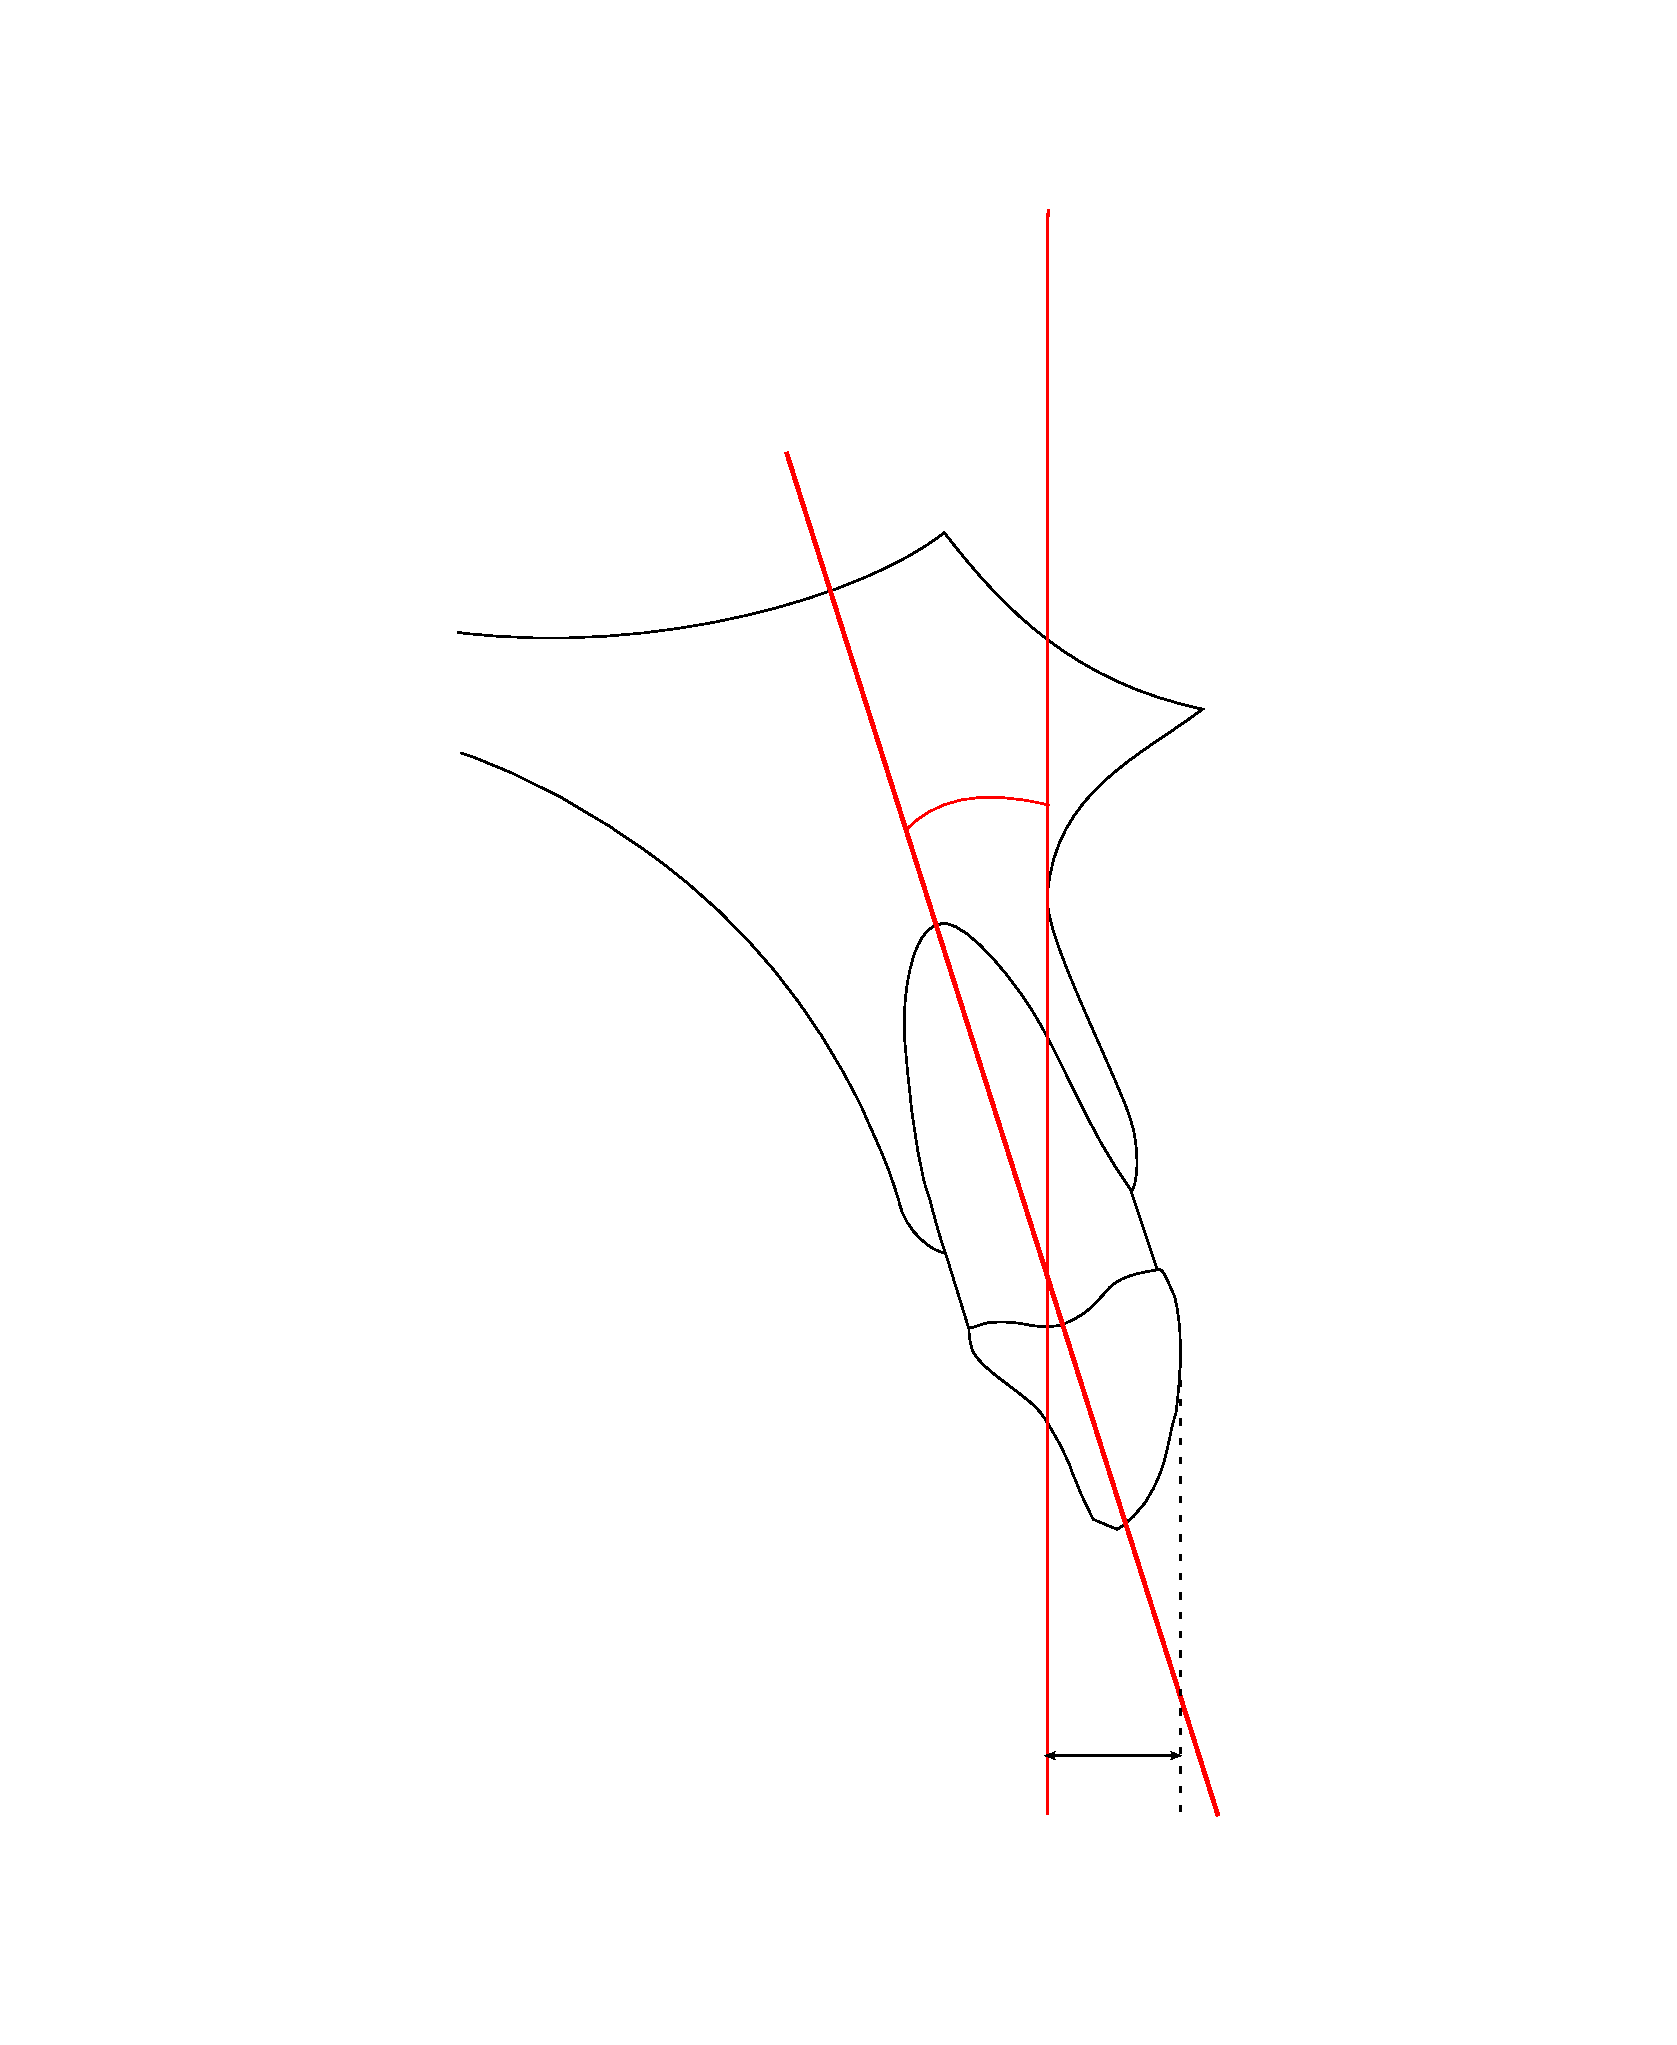
\includegraphics[width=.4\textwidth]{./images/steiner_incisale.pdf}}
 % steiner_incisale.jpg: 1006x1227 pixel, 72dpi, 35.49x43.29 cm, bb=0 0 1006 1227
 \caption{Posizione e angolazione ``ideale'' dell'incisivo superiore secondo Steiner}
 \label{fig:steiner_incisivo_superiore}
\end{wrapfigure}

\section{Analisi dentale}
\begin{table}[h]
%\footnotesize
\begin{tabularx}{\textwidth}{>{\bfseries}lXc}
\toprule
 & Punti di riferimento & Valore medio \\
\cmidrule(r){2-3}
Ang. occl.-inc. sup. & piano occlusale -- asse maggiore inc. sup. & 60° $\pm$ 2° \\
Inclinaz. inc. sup. & \piano{N}{A} -- asse maggiore inc. sup. & 22° \\
Posiz. inc. sup. & \piano{N}{A} -- superficie labiale inc. sup. & 4mm \\
Ang. occl.-inc. inf. & piano occlusale -- asse maggiore inc. inf. & 70° $\pm$ 3° \\
Inclinaz. inc. inf. & \piano{N}{B} -- asse maggiore inc. inf. & 25° \\
Posiz. inc. inf. & \piano{N}{B} -- superficie labiale inc. inf. & 4mm \\
Angolo interincis. & assi maggiori incisivi & 130° $\pm$ 5° \\
Angolo occl.-mol. sup. & piano occlusale -- asse maggiore sesto sup. & 90° $\pm$ 3° \\
%Angolo bimolare inf. & assi maggiori settimo e ottavo inf. & < 10° \\
\bottomrule
\end{tabularx}
\end{table}

Solitamente l'analisi dentale serve a confermare le valutazioni cliniche già compiute. D'altro canto, esistono numerosi casi in cui le valutazioni radiografiche differiscono notevolmente da quelle cliniche.

\paragraph{Posizione incisivo superiore}
La posizione degli incisivi superiori viene determinata correlando i denti alla linea \punto{N}-\punto{A}. È possibile considerare due valori: il primo riguarda l'angolazione dell'asse del dente e viene calcolato misurando il valore in gradi dell'angolo tra \punto{N}-\punto{A} e l'asse del dente. Il secondo valuta il posizionamento relativo, misurato in millimetri tra \punto{N}-\punto{A} e la superficie più labiale.

Usando questo metodo, gli incisivi centrali superiori dovrebbero essere posizionati in modo tale da avere la superficie più labiale ad una distanza di 4mm dalla linea, e un'inclinazione di 22°.

La sola valutazione dell'angolazione dell'incisivo superiore non è infatti sufficiente a dare un giudizio sulla posizione dei denti: potrebbe infatti capitare che l'angolazione sia corretta, ma che il dente sia traslato in avanti o indietro rispetto alla linea \punto{N}-\punto{A} (fig.~\ref{fig:steiner_traslazione}).

Allo stesso modo, la sola rilevazione della distanza millimetrica della superficie più labiale non è sufficiente. Non è difficile immaginare un incisivo a 4mm di distanza, ma inclinato diversamente (fig.~\ref{fig:steiner_rotazione}).

Giannì introdusse un ulteriore angolo, in rapporto al piano occlusale, con un valore medio di 60° $\pm$ 2°.

\begin{figure}[p!]
\subfloat[][]
   {\label{fig:steiner_traslazione}\fbox{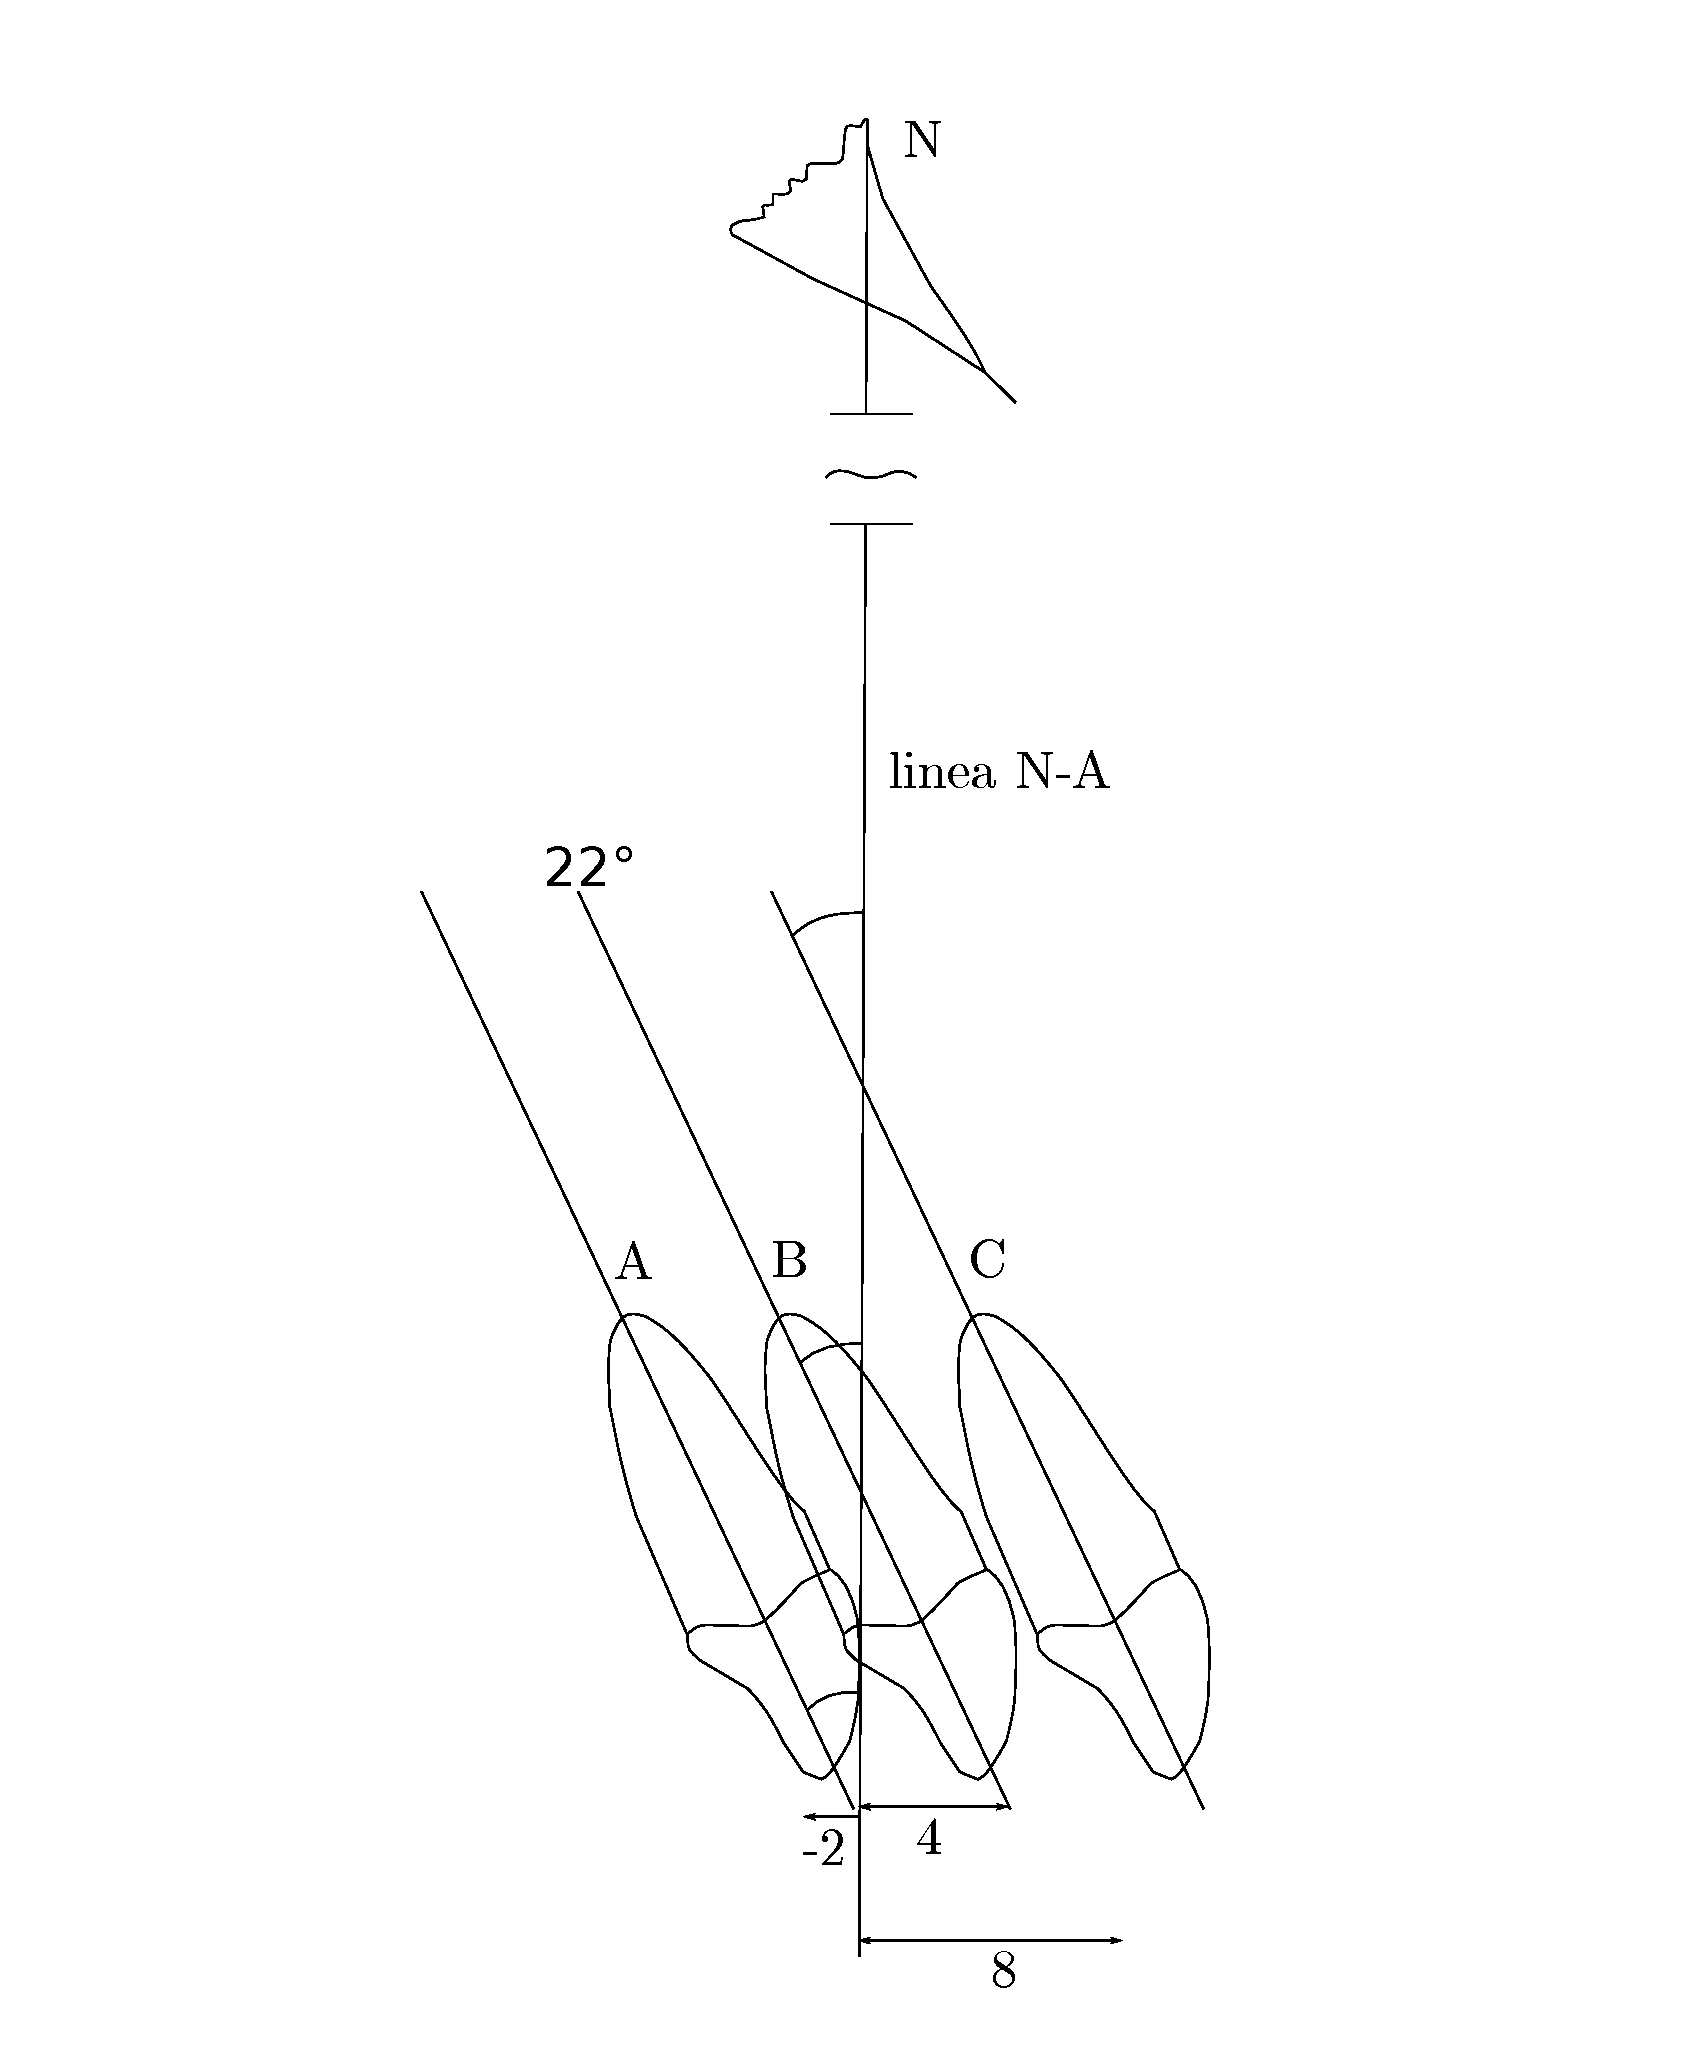
\includegraphics[width=.45\textwidth]{./images/steiner_incisivo_traslazione.pdf}}} \quad
\subfloat[][]
   {\label{fig:steiner_rotazione}\fbox{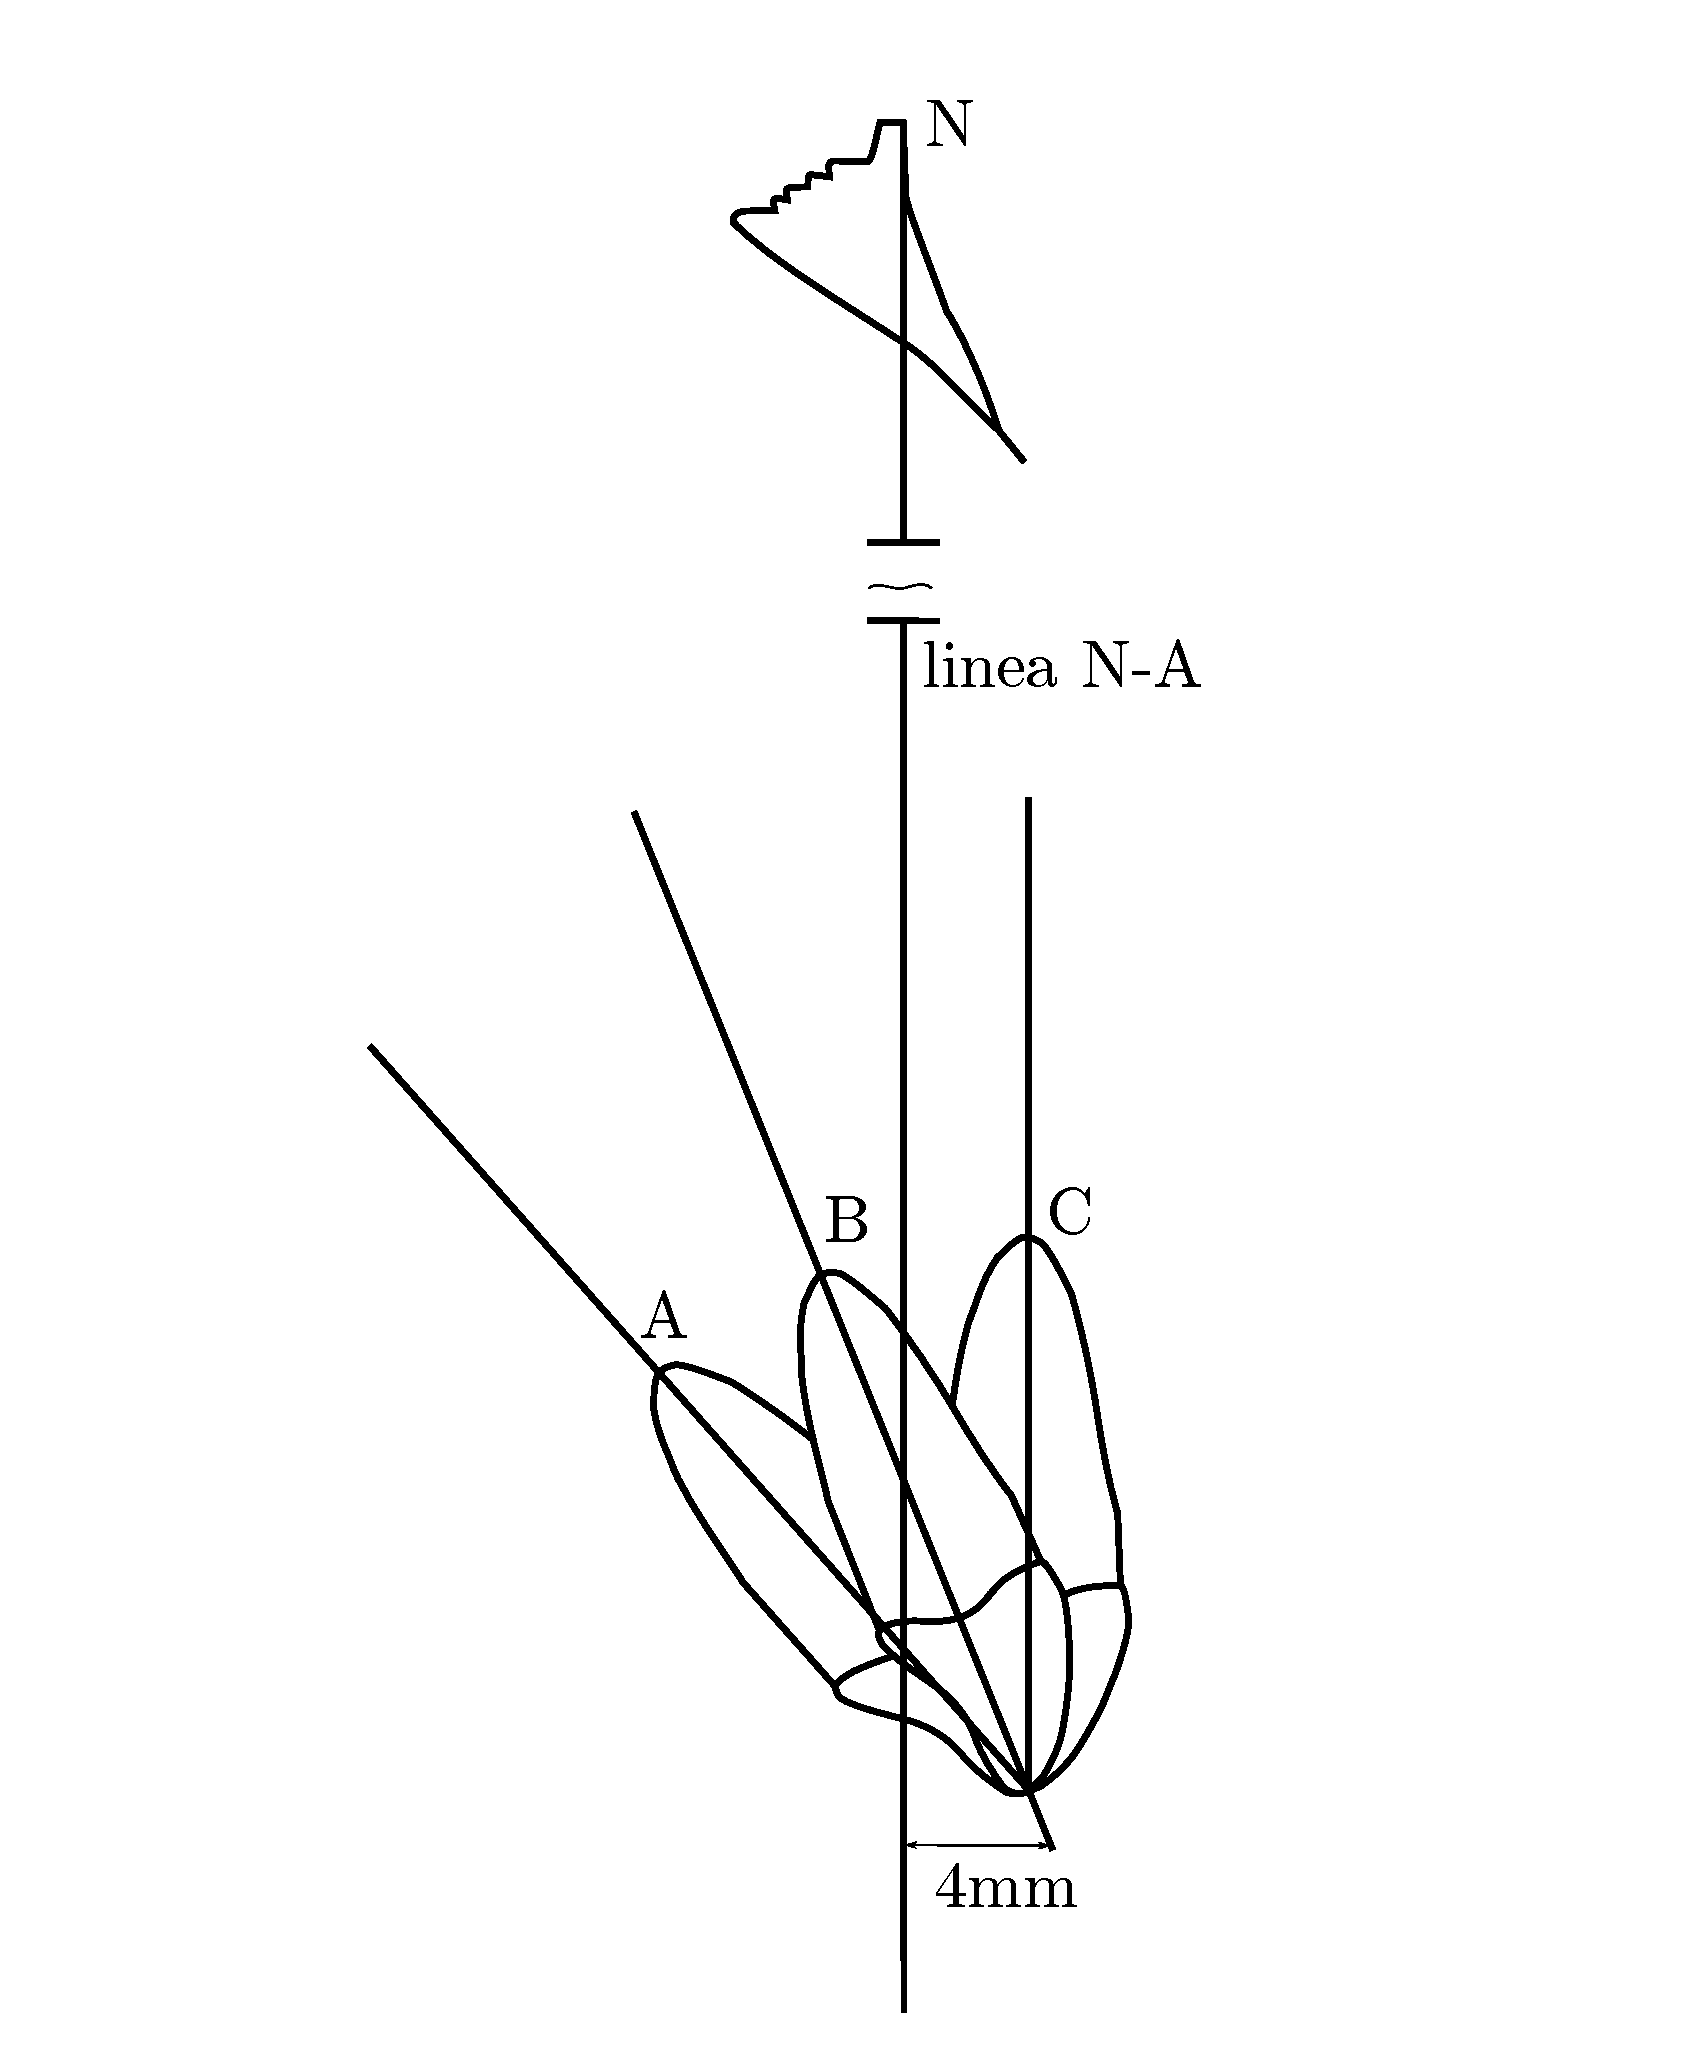
\includegraphics[width=.45\textwidth]{./images/steiner_incisivo_rotazione.pdf}}}
 \centering
 % steiner_sna.jpg: 1024x988 pixel, 72dpi, 36.12x34.85 cm, bb=0 0 1024 988
 \caption{Inclinazione e posizione dell'incisivo superiore, in relazione alla linea \punto{N}-\punto{A}: \subref{fig:steiner_traslazione} inclinazione corretta, ma posizione variabile; \subref{fig:steiner_rotazione} posizione corretta, ma inclinazione variabile.}
 \label{fig:steiner_incisivo_rototraslazione}
\end{figure}

\paragraph{Posizione incisivo inferiore}
Allo stesso modo che per l'incisivo superiore, per valutare la posizione dell'incisivo inferiore si misurano la distanza millimetrica tra superficie più labiale e linea \punto{N}-\punto{B}, e valore angolare tra questa e l'asse maggiore del dente. Anche in questo caso, Giannì propose la valutazione angolare rispetto al piano occlusale.

\begin{figure}[p!]
\centering
\begin{minipage}{.44\textwidth}
 \centering
 \fbox{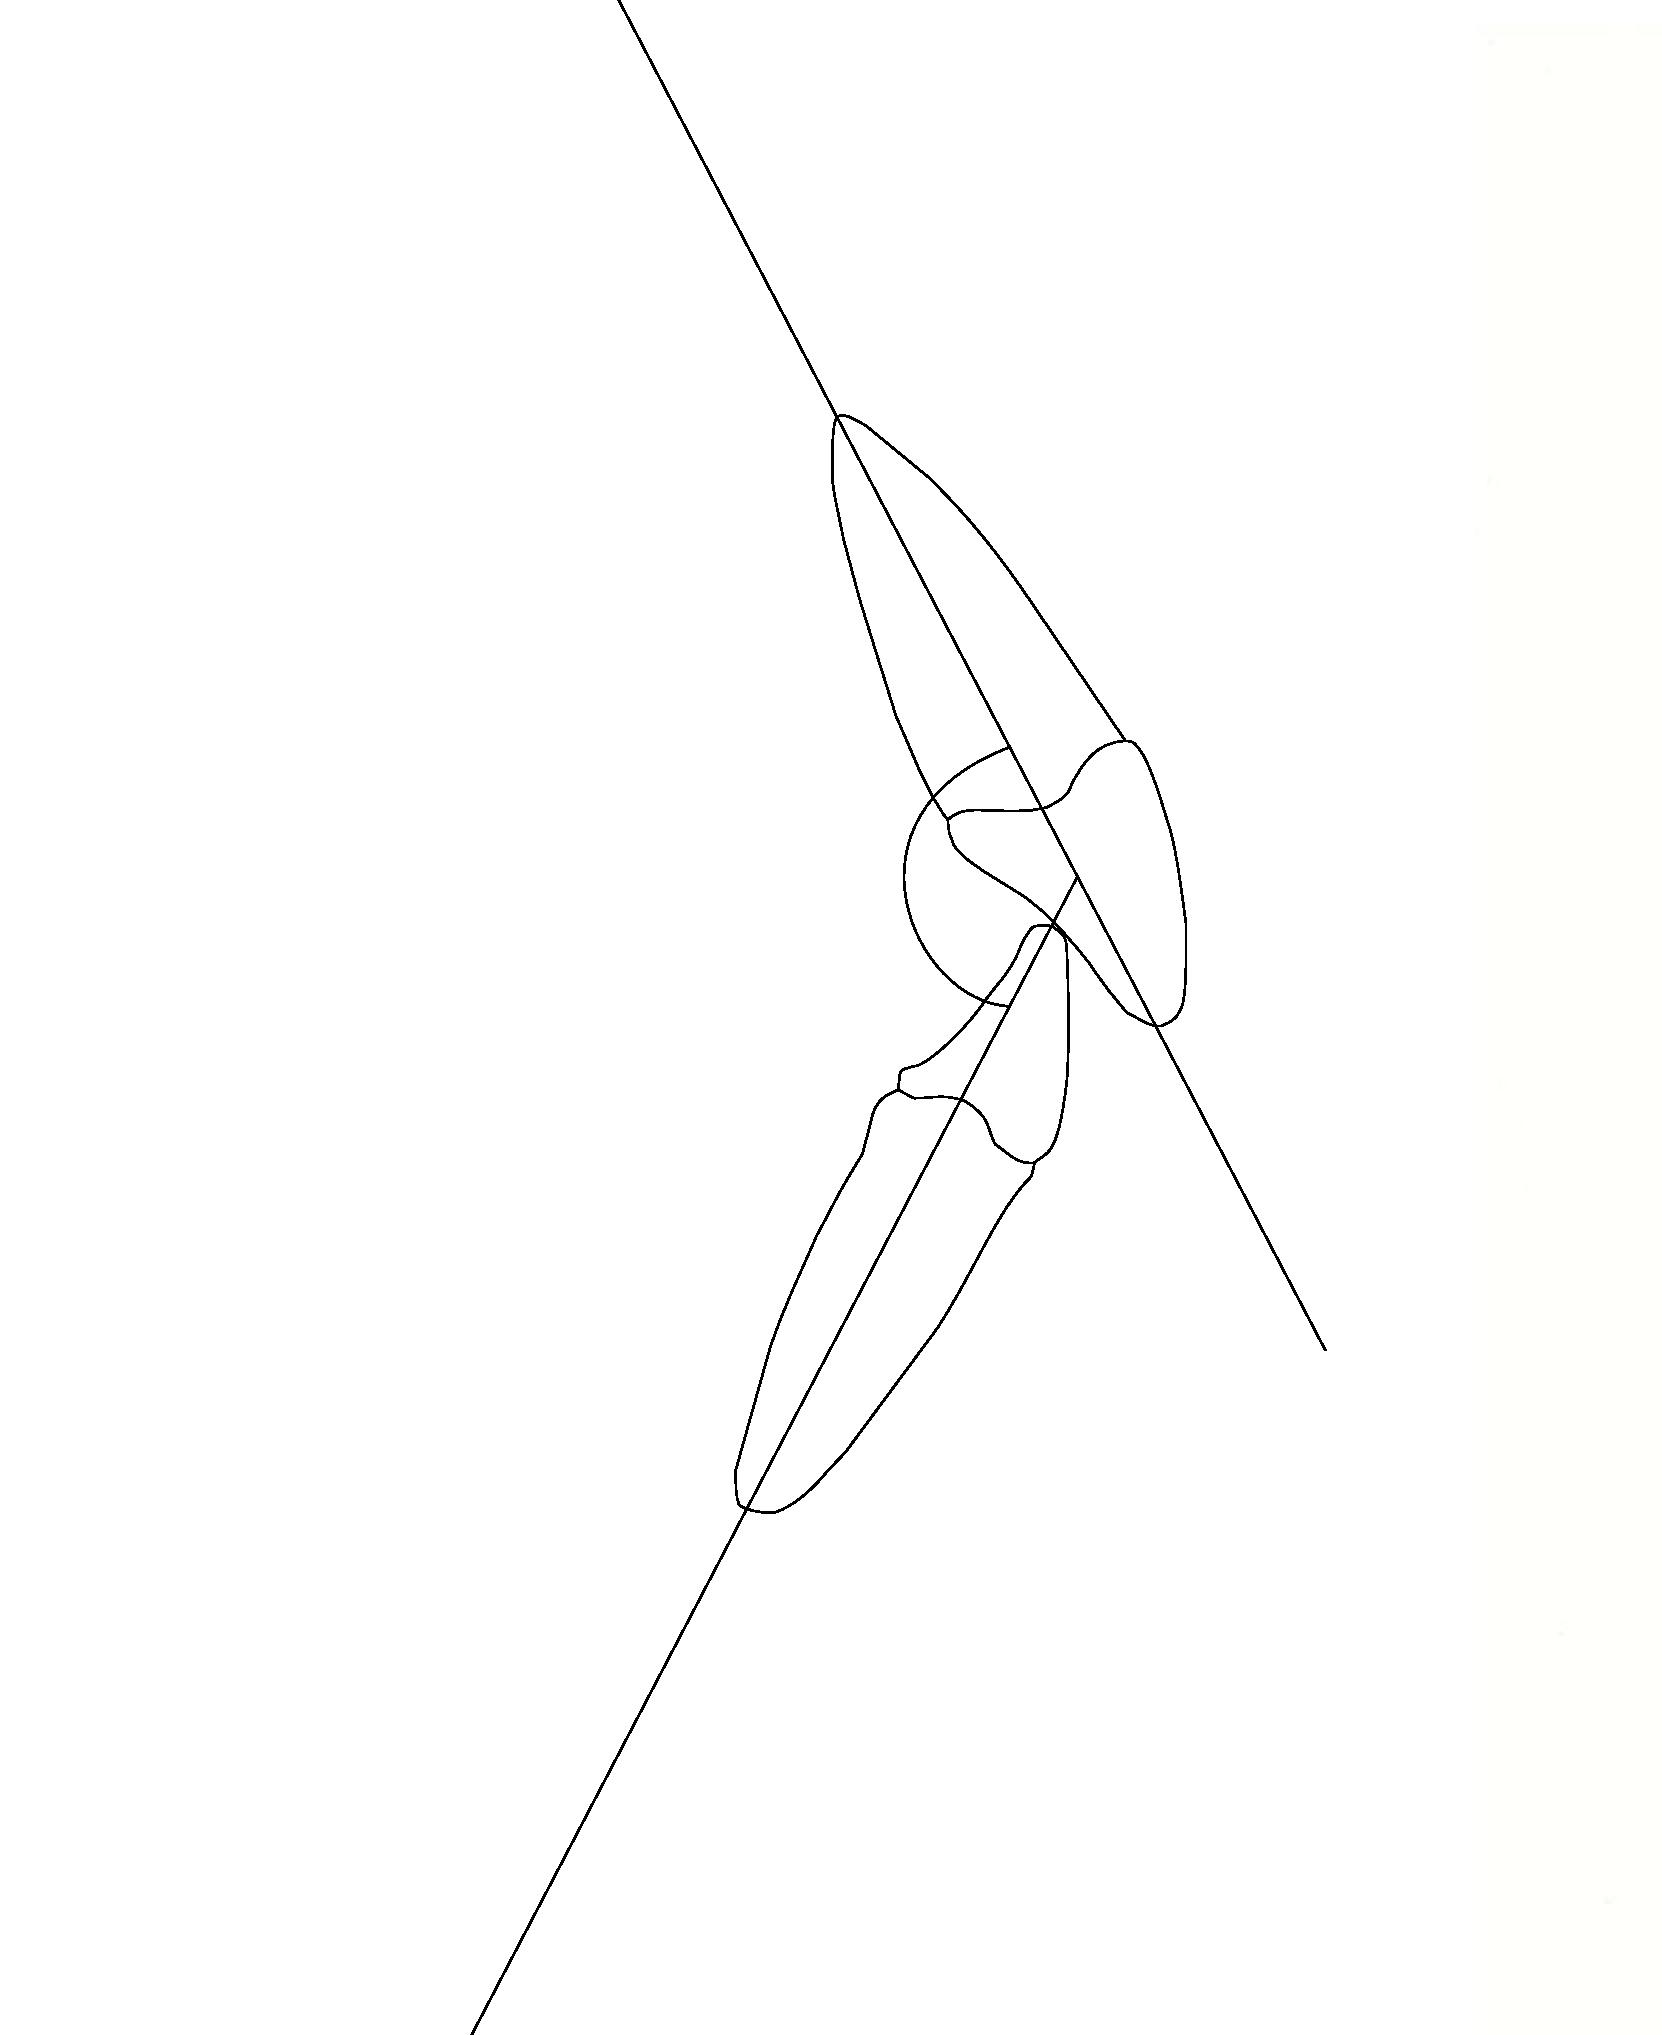
\includegraphics[width=.95\textwidth]{./images/steiner_interincisale.pdf}}
 \caption{Angolo interincisale}
 \label{fig:steiner_interincisale}
\end{minipage}\quad\quad
\begin{minipage}{.44\textwidth}
 \centering
 \fbox{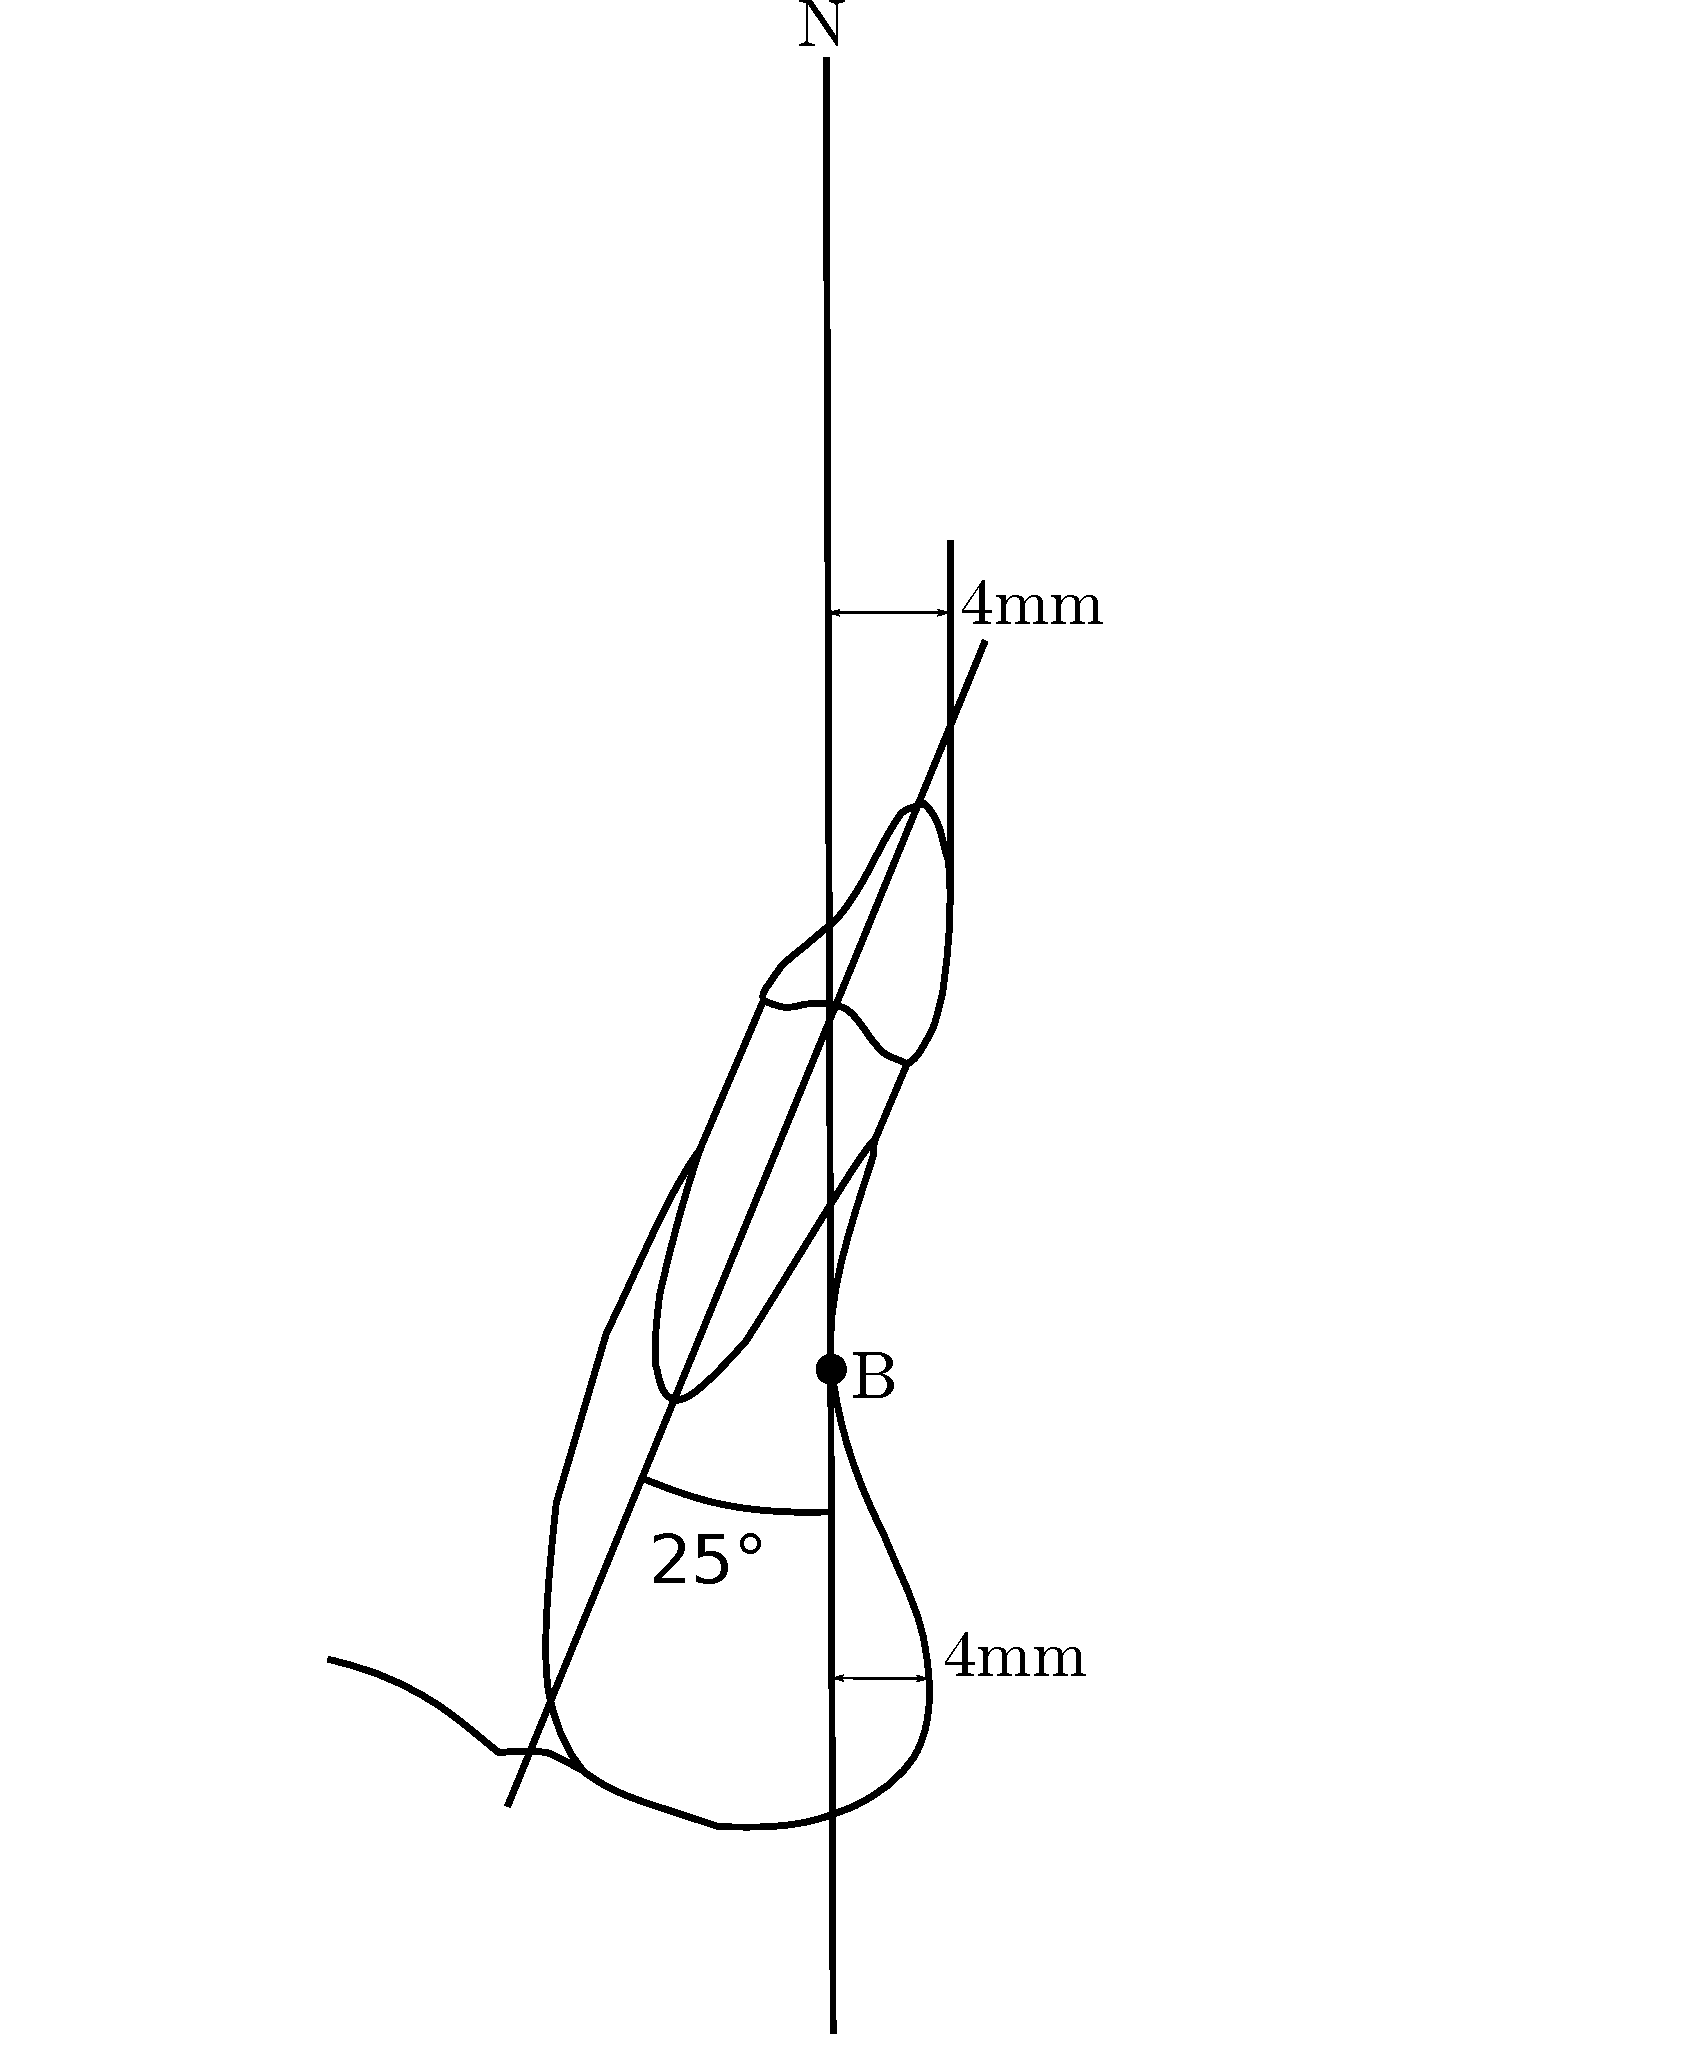
\includegraphics[width=.95\textwidth]{./images/steiner_incisivo_inferiore.pdf}}
 \caption{Rapporto tra incisivo inferiore, linea \punto{N}-\punto{B} e mento.}
 \label{fig:steiner_incisivo_inferiore}
\end{minipage}
\end{figure}

\paragraph{Angolo interincisale}
L'angolo interincisale (fig.~\vref{fig:steiner_interincisale}) mette in relazione la posizione degli incisivi centrali superiore e inferiore. Il valore medio è 130° $\pm$ 5°: valori minori o maggiori indicano una necessità di variazione dell'inclinazione di uno o entrambi gli incisivi. Nell'ipertono muscolare il valore angolare tende ad aumentare, e gli incisivi tendono alla palatinizzazione; viceversa nell'ipotono muscolare il valore angolare tende a diminuire, e gli incisivi tendono a vestibolarizzarsi.

\paragraph{Angolo occluso-molare superiore} introdotto da Giannì, obiettiva l'inclinazione del primo molare superiore rispetto al piano occlusale. Ha un valore medio di 90° $\pm$ 3°.

\paragraph{Posizione sagittale primo molare superiore} secondo Giannì. Viene valutata al fine di evidenziare la presenza di una mesializzazione dell'arcata dentaria superiore. Tale valutazione è basata sui rapporti tra il primo molare superiore e la retta \piano{S}{Gn}. Nella Classe I scheletrica, tale retta passa per il centro della cuspide mesio-vestibolare del primo molare superiore. La posizione del molare, però, dev'essere considerata in rapporto alla posizione delle basi ossee: è necessario quindi considerare anche l'angolo \angolo{ANB}. Per esempio, per un \angolo{ANB} di 5° (Classe II), è normale una mesializzazione del primo molare di 3mm: con la riduzione in Classe I (\angolo{ANB} di 2°), si avrà un avanzamento mandibolare di 3mm, per cui il molare sarà ben posizionato.

%\paragraph{Angolo bimolare inferiore} anch'esso introdotto da Giannì, è l'angolo formato tra l'asse maggiore del secondo molare inferiore e l'asse maggiore del terzo molare inferiore. La sua valutazione orienta sul tipo di eruzione del terzo molare inferiore. Un valore inferiore a 10° è indice favorevole all'eruzione e all'allineamento in arcata del terzo molare; con un valore superiore a 20° si ha, nella maggioranza dei casi, la disodontiasi del terzo molare.

\paragraph{Distanza tra \punto{N}-\punto{B} e il mento}
Visto il generoso contributo del mento al profilo facciale, è necessario tenerlo in considerazione nella valutazione cefalometrica. Il grado di prominenza del mento contribuisce al posizionamento dei denti in arcata. Idealmente, secondo Holdaway\footcite{Holdaway1956}, la distanza tra la linea \punto{N}-\punto{B} e il mento dovrebbe essere uguale alla distanza tra la stessa linea e la superficie più labiale dell'incisivo inferiore (fig.~\ref{fig:steiner_incisivo_inferiore}). Una discrepanza di 2mm tra questi valori è accettabile, 3mm è meno desiderabile, ma ancora tollerabile. Una discrepanza superiore ai 4mm, invece, richiede generalmente un intervento.

\section{Analisi dei tessuti molli}
L'analisi dei tessuti molli consiste in una registrazione grafica delle osservazioni cliniche effettuate durante l'esame del paziente. Essa include una valutazione dell'adattamento dei tessuti al profilo osseo sottostante, tenendo in considerazione dimensioni, forma e postura delle labbra. Viene inoltre analizzato lo spessore dei tessuti molli sulla sinfisi mentoniera e sulla struttura nasale, e al loro rapporto con la parte inferiore della faccia.

\begin{figure}[h!]
 \centering
 \fbox{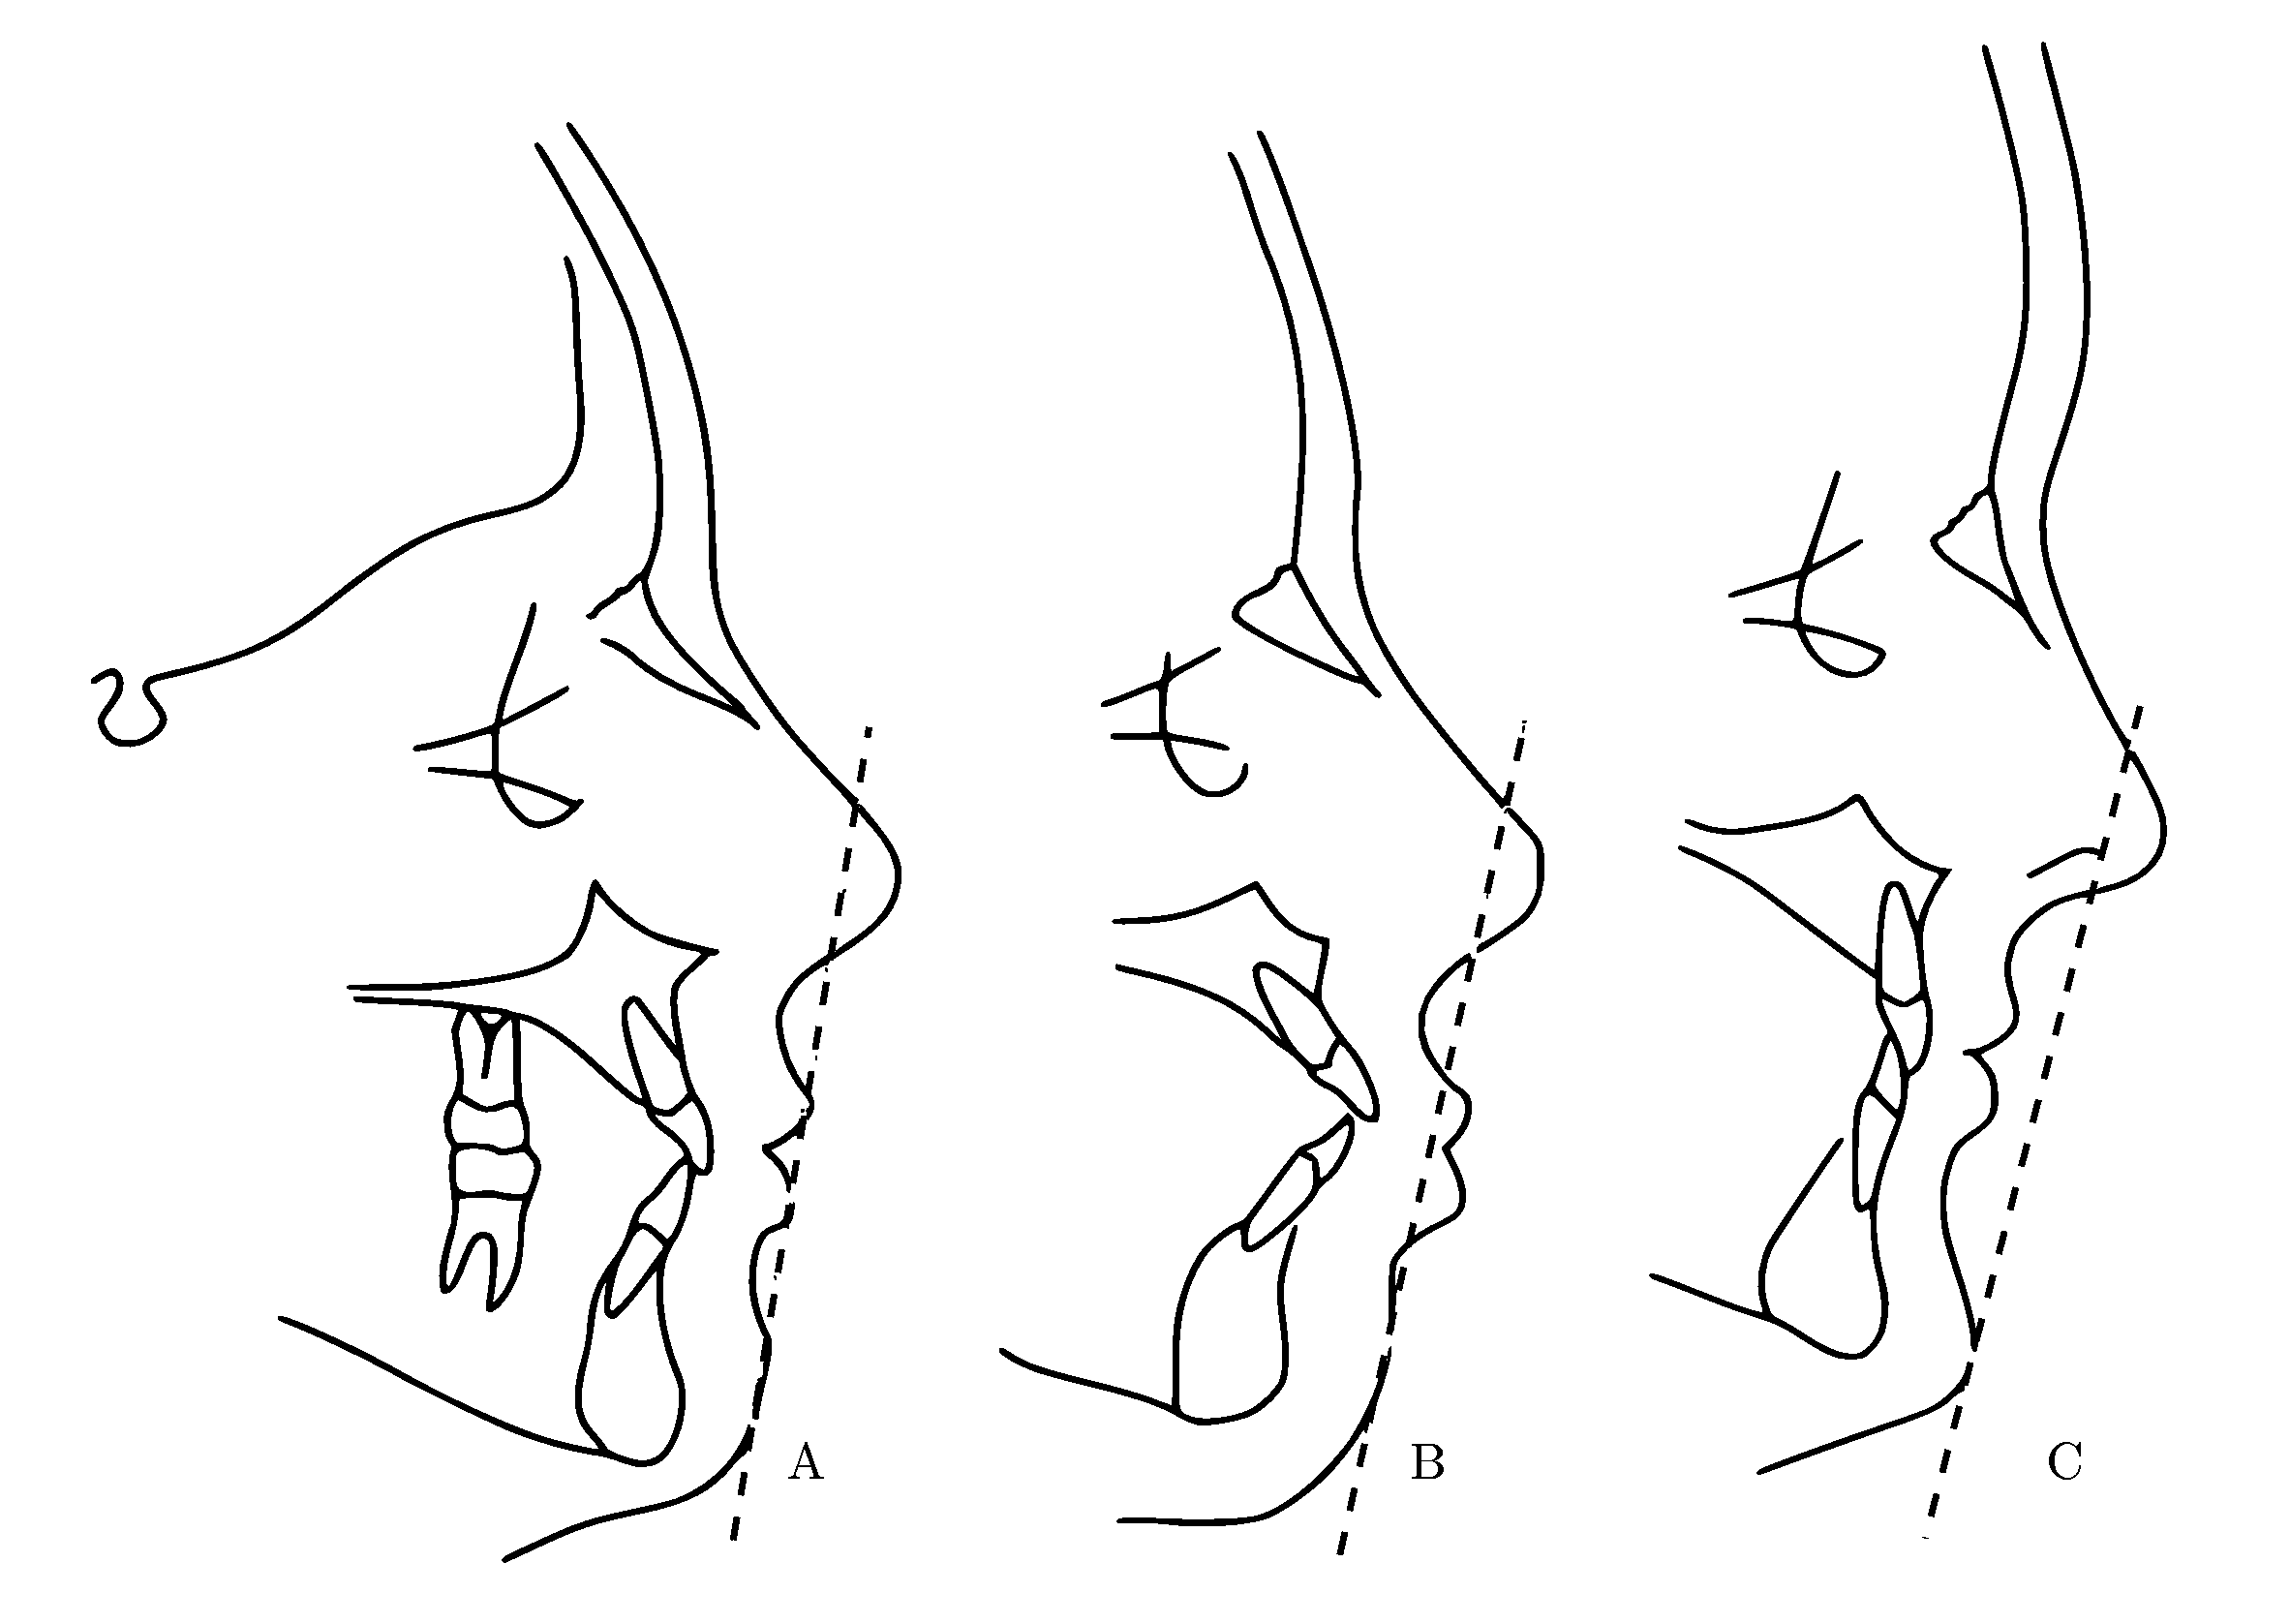
\includegraphics[width=.75\textwidth]{./images/steiner_linea_s.pdf}}
 % steiner_linea_s.jpg: 1419x1006 pixel, 72dpi, 50.06x35.49 cm, bb=0 0 1419 1006
 \caption{Linea S di Steiner: (a) labbra in equilibrio, (b) labbra protruse, (c) profilo retruso}
 \label{fig:steiner_linea_s}
\end{figure}

Steiner, Ricketts, Holdaway e Meddifield hanno sviluppato criteri e linee di riferimento per l'armonia del profilo facciale. Sebbene non possa esistere un concetto uniforme di cosa costituisca un profilo ideale, la \textit{linea S} di Steiner (fig.~\ref{fig:steiner_linea_s}) è molto usata nell'ortodonzia odierna per determinare l'equilibrio dei tessuti molli facciali. Le labbra, secondo Steiner, dovrebbero toccare una linea passante dal contorno del mento al punto mediano di una S formata dal bordo inferiore del naso. Questa linea viene chiamata \textit{linea S}.

Labbra posizionate oltre questa linea tendono alla protrusione, e il trattamento richiesto solitamente prevede un retroposizionamento dentale o scheletrico. Se invece le labbra sono posizionate posteriormente, il paziente ha un profilo generalmente interpretato come ``concavo'', la cui correzione ortodontica prevede un avanzamento dei denti, causando un avanzamento delle labbra.

Giannì effettua una modifica alla linea estetica di Steiner, tale da renderla attendibile nei casi di eccessivo o tardivo accrescimento della piramide nasale, secondo le critiche di Müller\footcite{Mueller1969}. Egli, infatti, considera come punto di mezzo del sotto-setto nasale (il ``centro'' della S secondo Steiner) il punto di mezzo di una linea perpendicolare alla retta \piano{N}{AN} (\punto{AN} è l'apice dell'osso nasale) passante per \punto{PS} (piede del sotto-setto nasale).

Nel caso in cui esistano le indicazioni clinica all'estrazione di premolari, la linea estetica è un'importante guida nella scelta dei premolari da estrarre. Se, infatti, il labbro dell'arcata coinvolta oltrepassa la linea estetica, allora è giustificata l'estrazione dei due primi premolari; è giustificata invece l'estrazione dei secondi premolari nel caso in cui il labbro coincida con la linea estetica. La spiegazione di questo ragionamento va ricercata nella stretta correlazione tra la zona delle estrazioni e il collasso del labbro: più le estrazioni sono posteriori, meno il labbro collassa e, pertanto, meno il profilo si modifica.
